\documentclass[a4paper,10pt]{scrartcl}
%encodings
\usepackage[utf8]{inputenc}
\usepackage[english]{babel}
\usepackage[T1]{fontenc}
%colors, hyperrefs
\usepackage{color}
\usepackage{url}
\usepackage[pdftex,pdfauthor={J\"org Behrmann, Anika Haller},pdftitle={Ma4: X-Ray Photoelectron Spectroscopy (XPS)}]{hyperref}
%figures and subfigures
\usepackage[pdftex]{graphicx}
\usepackage{subfigure}
%better tables
\usepackage{tabularx}
\usepackage{booktabs}
\usepackage{multirow}
%math stuff
\usepackage{amsmath}
\usepackage{amsthm}
\usepackage{amsfonts}
\usepackage{IEEEtrantools}
\usepackage[square,comma,numbers,sort&compress]{natbib}
%shiny stuff
\usepackage[babel]{microtype}
\DisableLigatures{encoding=T1,family=tt*}

\usepackage{verbatim}

\begin{document}

\title{Ma4: X-Ray Photoelectron Spectroscopy (XPS)}
\author{J\"org Behrmann\footnote{behrmann@physik.fu-berlin.de} \qquad Anika Haller\footnote{halleran@zedat.fu-berlin.de}}
\date{02.01.2012}
\maketitle
\tableofcontents
\thispagestyle{empty}

\section{Introduction}

X-Ray Photoelectron Spectroscopy (XPS) is an electron spectroscopy technique in which a sample is probed with highly-energetic photons in the X-ray spectrum. These photons can induce a wide range of different processed in the sample, e.g. excitation of valence electrongs, excitation of Auger electrons, plasmon excitation, etc., and resulting emitted electrons resolved for their kinetic energy give considerable information about the band structure of the material.

\subsection{Universal Curve of Escape Depth}

Figure~\ref{fig:ucurve} shows the universal curve of electron escape depth, which shows that that the depth from which an incoming electron can escape from a surface again is only dependent on the electron's energy and thus more or less independent of the material. This universal curve can be obtained on theoretical grounds by considering that first for increasing energy (up to $70\,$eV) more and more interaction modes, e.g. phonon modes, become available as potential scatterers to the incoming electron, which decreases the particles mean free path. Whereas for even higher energies the excess energy can be used to penetrate the material further.

As the typical kinetic energies of electrons in XPS are between $20$ and $100\,$eV, we see in figure~\ref{fig:ucurve}, that this technique is very surface sensitive.

\begin{figure}
\centering
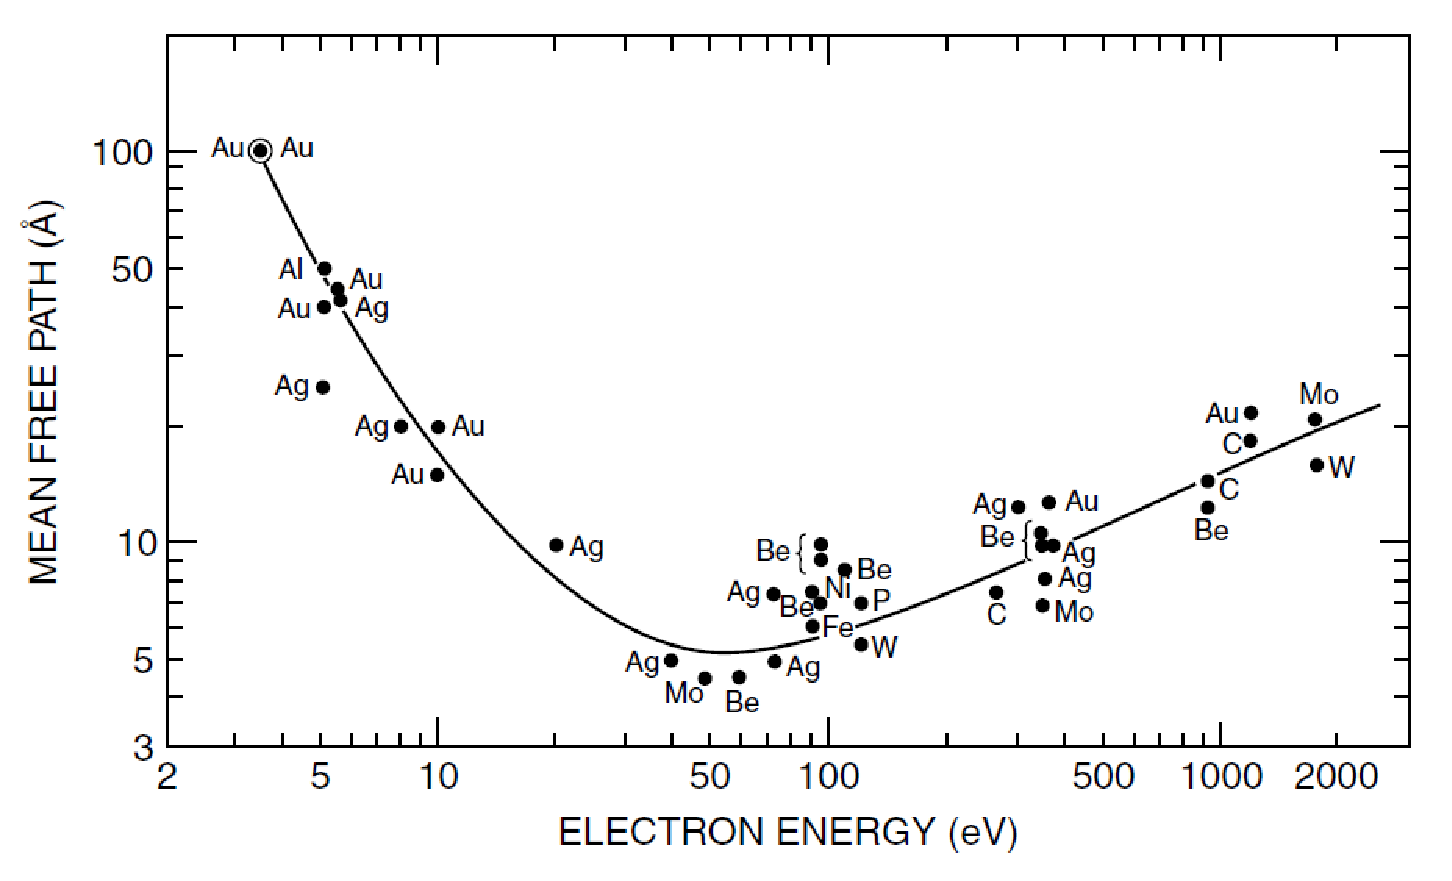
\includegraphics[scale=0.4]{img/ucurve}
\caption{Universal curve of electron escape depth \label{fig:ucurve}}
\end{figure}

\subsection{The XPS spectrum}

Figure~\ref{fig:spectrum} shows a sample XPS spectrum, where (a) are peaks from emissions of core level electrons, (b) are peaks from Auger processes, (c) are peaks from emission of valence band electrons and (d) are peaks secondary electron electron excitation and inelastic scattering processed.

\begin{figure}
\centering
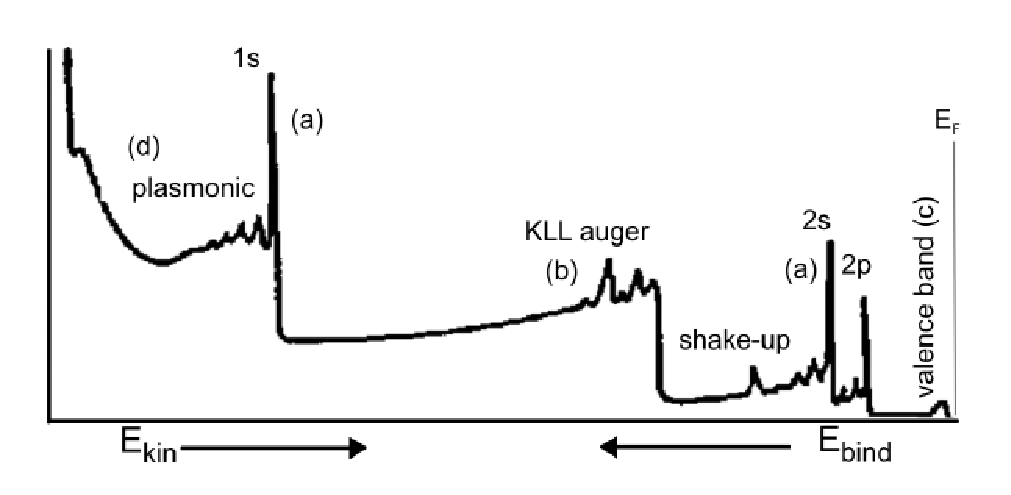
\includegraphics[scale=0.4]{img/spectrum}
\caption{Sample XPS spectrum \label{fig:spectrum}}
\end{figure}

\subsubsection{The Photoelectric Effect}

The grand strucuture of the XPS spectrum is supplied by the multiplett structure (as described in the following section) that is probed by the simple photoelectric effect.

In the photoelectric effect a single electron absorbs a single photon and is excited in the vacuum with the kineti energy:
\begin{equation}
E_{kin} = \hbar \nu - E_{B} - \Phi,
\end{equation}
where the first term on the right-hand side gives the energy of the incoming photon, the second term $E_{B}$ gives the binding energy of the electron measured with respect to the Fermi energy and the last term $\Phi$ gives the work function of the material, which is the difference between the Fermi and vacuum level, i.e. the minimum energy to excite an electron from the material.

The binding energy of a material is different to the one of a free atom of this element. It is given by
\begin{equation}
E_{B} = E_{B,atom} + \Delta E_{chem} + \Delta E_{lattice} + \Delta E_{ref}, \label{eq:binding}
\end{equation}
where $\Delta E_{chem}$ gives the chemical shift, due to neighbouring atoms, $\Delta E_{lattice}$ gives the difference due electrostatic interactions in the lattice (usually called the Madelung constant) and $\Delta E_{rel}$ subsumes many-body effects in the final 1-hole state.

\subsection{Spin-Orbit Coupling}

To fully describe an electron's energy in an atom---and by that the multiplet structure of the XPS spectrum---one has to account for magnetic moments of the electron. Each electron has a magnetic moment due to its orbital movement in the atom and another one due to its spin. All of these magnetic moments of all electrons interact and lead to energy shifts in the spectra. For light atoms the spin-orbit interaction can be approximated by an interaction of the total angular momentum and the total spin (L-S-coupling), which is possible when the coupling of individual spins and orbital angular momenta is negligible. The part of the Hamiltonian describing spin-orbit coupling is then given by
\begin{equation}
H_{SL} = - \frac{\mu_B}{\hbar m_e e c^2}\frac{1}{r}\frac{\partial V(r)}{\partial r} \boldsymbol{L}\cdot\boldsymbol{S},
\end{equation}
where $\mu_B$ is the Bohr magneton, $m_e$ is the electron mass, $e$ is the elementary charge, $c$ is the speed of light, $V$ is the core potential and $r$ is the distance of the electron to the nucleus.
For heavier atoms the coupling between individual spin and orbital momenta is non-negligible and a better approximation is the coupling of individual total angular moment $J_i=L_i+S_i$, this is called J-J-coupling. 

As our samples will be made of heavier elements, J-J-Coupling is the better approximation. Thus all emission lines of full electron shells in the ground state will split in doublets for $(l+\tfrac{1}{2})$ and $(l-\tfrac{1}{2})$. In principle for s-shells with $l=0$ no splitting would occur, but an effect called magnetic spin-spin exchange splitting, leads to a doublet splitting of s-shells through the interaction partially filled shells.


\subsubsection{Inner-Shell Excitations and the Auger Effect}

If a core electron is excited, one possible relaxation process is the emission of an Auger electron. In this relaxation process an electron from a higher shell fills the core hole and the emitted photon is absorbed by another electron in a higher shell that is thus excited in the continuum. The resulting atom is doubly ionized. 

The energy of the emitted Auger electron is given by
\begin{equation}
E_{kin} = E(K)-E(L)-E'(L') = E(K)-E(L)-E(L')-C(LL',T)+R
\end{equation}
where the $E(K)$ is the binding energy of the core electron, $E(L)$ is the binding energy of the electron filling the core hole. $E'(L')$ is the effective binding energy of the electron that is emitted as Auger electron. The effective binding energy consists of the binding energy of the shell $E(L')$, a coupling energy between the holes at $L$ and $L'$ and the final state $T$ and a so-called electronic relaxation $R$. It is important to note that the kinetic energy of the Auger electron is only dependent on the participating states of the Auger process and not on the energy of the particle that initially excites the core electron.

\subsubsection{Plasmons}

A plasmon is a quasi-particle coming up in condensed matter, describing quantized plasma oscillations, i.e. oscillations of the electron gas as a whole. The excitation energy of plasmons is specific to all materials and are given by the materials plasma frequency, both of which are tabulated and can be looked up. 

For a free electron gas the bulk plasma frequency is given by
\begin{equation}
\omega_{b} = \sqrt{\frac{e^2 n}{m_e \epsilon_0}},
\end{equation}
where $e$ is the elementary charge, $\epsilon_0$ the permittivity of free space, $m_e$ the mass of the electron and $n$ the conduction electron density. Apart from the 3-dimensional case also surface plasmons, excitations of the electron gas restricted to the surface, can be excited.

An electron having excited one or more plasmons is said to have suffered plasmon loss. This is one reasion for satelites to ``real'' peaks in spectra.

\section{Experimental Setup}

In this section we will describe shortly the machinery and techniques used in this experiment. A schematic of the setup is shown in figure~\ref{fig:setup}.

\begin{figure}
\centering
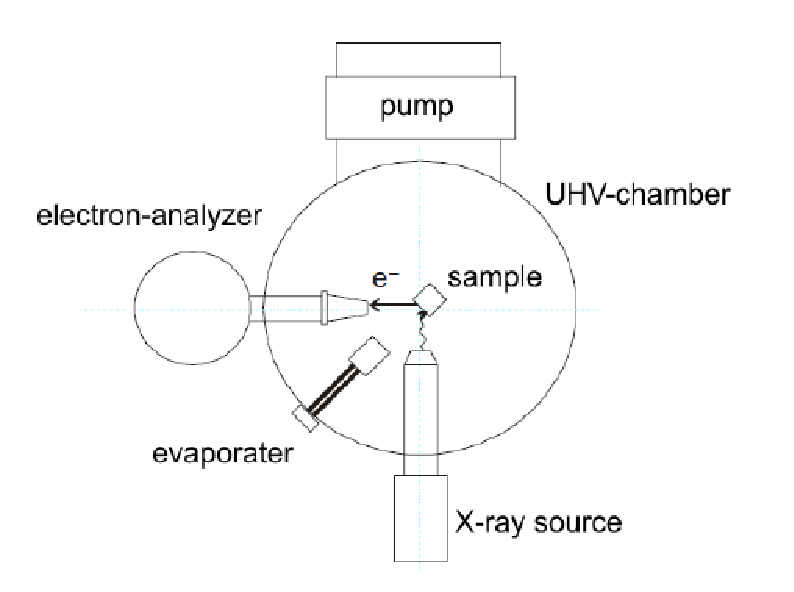
\includegraphics[scale=0.4]{img/setup}
\caption{Schematic setup of the experimen.t \label{fig:setup}}
\end{figure}


\subsection{Ultra High Vacuum (UHV)}

This experiment needs an ultra high vacuum environment for two reasons. First, electrons have very short mean free path in matter, as can be seen in figure~\ref{fig:ucurve}. Second, the higher the pressure the faster gas atoms from the rest atmosphere in the chamber adsorb to the sample, this is again unwanted, as XPS is a very surface sensitive technique and assertions about bulk properties of samples can, if ever, only be made from properties of atomically clean surfaces.

The ultra high vacuum is usually obtained by the use of membrane, turbo molecular, ion getter pump and sublimation pumps, as well as baking of the chamber. This experiment uses a rotary vane pump to achieve a prevacuum of about $\sim 10^{-6}\,$mbar and based on that, a turbomolcular pump to achieve a vacuum of about $10^{-9}\,$mbar. The final pressure of about $10^{-10}\,$mbar is achieved through baking.

\paragraph{The Rotary Vane Pump} is a rather simple mechanical pump. In a cylinder a vane, pressed to the cylinder walls by springs, rotates and mechanically ``shovels'' out the gas.

\paragraph{The Turbomolecular Pump} is another type of mechanical pump. It consists of several stages of rotors and stators. The rotors are tilted blades rotating at a velocity approximately equal to that of the gas particles and the stators are stationary blades tilted in the other direction orthogonal to the rotors. The working principle of this pump is to transfer momentum to the gas particles in a way such that the particles are ``kicked'' out of the chamber; the tilt of the rotors is such that the momentum of the kicked particles points outward the chamber.

\paragraph{Baking} is the technique through which the final pressure is achieved. The remaining pressure achieved through the use of pumps is mainly due to water molecules still in the chamber. Due to teir polarity, these water molecules are usually located at the chamber walls. By cycles of heating and cooling of the chamber they can be pumped out. This procedure can take several days, which makes it of utmost importance to maintain the UHV after it is obtained.

\subsection{X-Ray Source}

The X-ray source used in this experiment is made of a filmanent from which electrons are emitted by thermal excitation. These electrons are then accelerated and hit an anode, either aluminum or magnesium, were they produce characteristic X-ray radiation by excitation of core level electrons in the anode and a continous X-ray spectrum through Bremsstrahlung.

The characteristic X-ray radition is filtered out by usage of an Aluminium window and only the continous spectrum is used of spectroscopy.

\subsection{Electron Energy Analyzer}

This experiment uses a hemispherical electron analyzer, as shown in figure~\ref{fig:analyzer}. The analyzer consists of two hemispherical capacitors between which an electric field is applied, thus changing the trajectory of electrons coming in through the first aperture. The strength of this field is varied such that only electrons in a certain energy range pass through the second aperture.

Before entering through the first aperture a pass voltage can be applied to the electrons, which is useful because most detectors are more accurate at lower energies, therefore a constant energy offset can be used to increase the accuracy of the measurement an order of magnitude.

The final electron detecter is a channeltron, which is a  continuous version of a dynode electron multiplier. The channeltron is basically a thin glass cone coated with a semiconducting material. The signal is amplified by emission of secondary electrons, which multiplies the number of electrons in the channeltron that finally arrive at the anode. The electron multiplication is usually of the order $10^6$ to $10^9$.

\begin{figure}
\centering
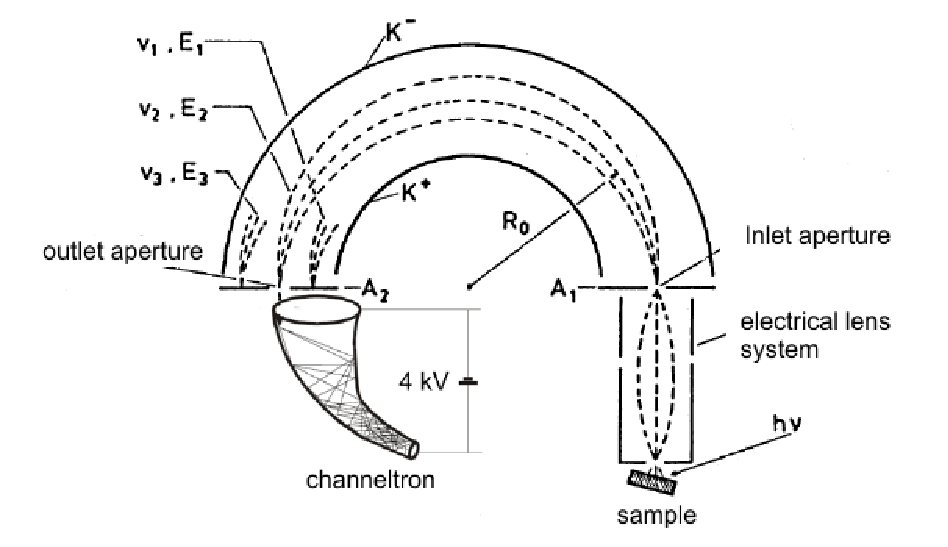
\includegraphics[scale=0.4]{img/analyzer}
\caption{Schematic of a hemispheric electron analyzer \label{fig:analyzer}}
\end{figure}

\section{Data Analysis}

\subsection{Silver}

\begin{figure}
\centering
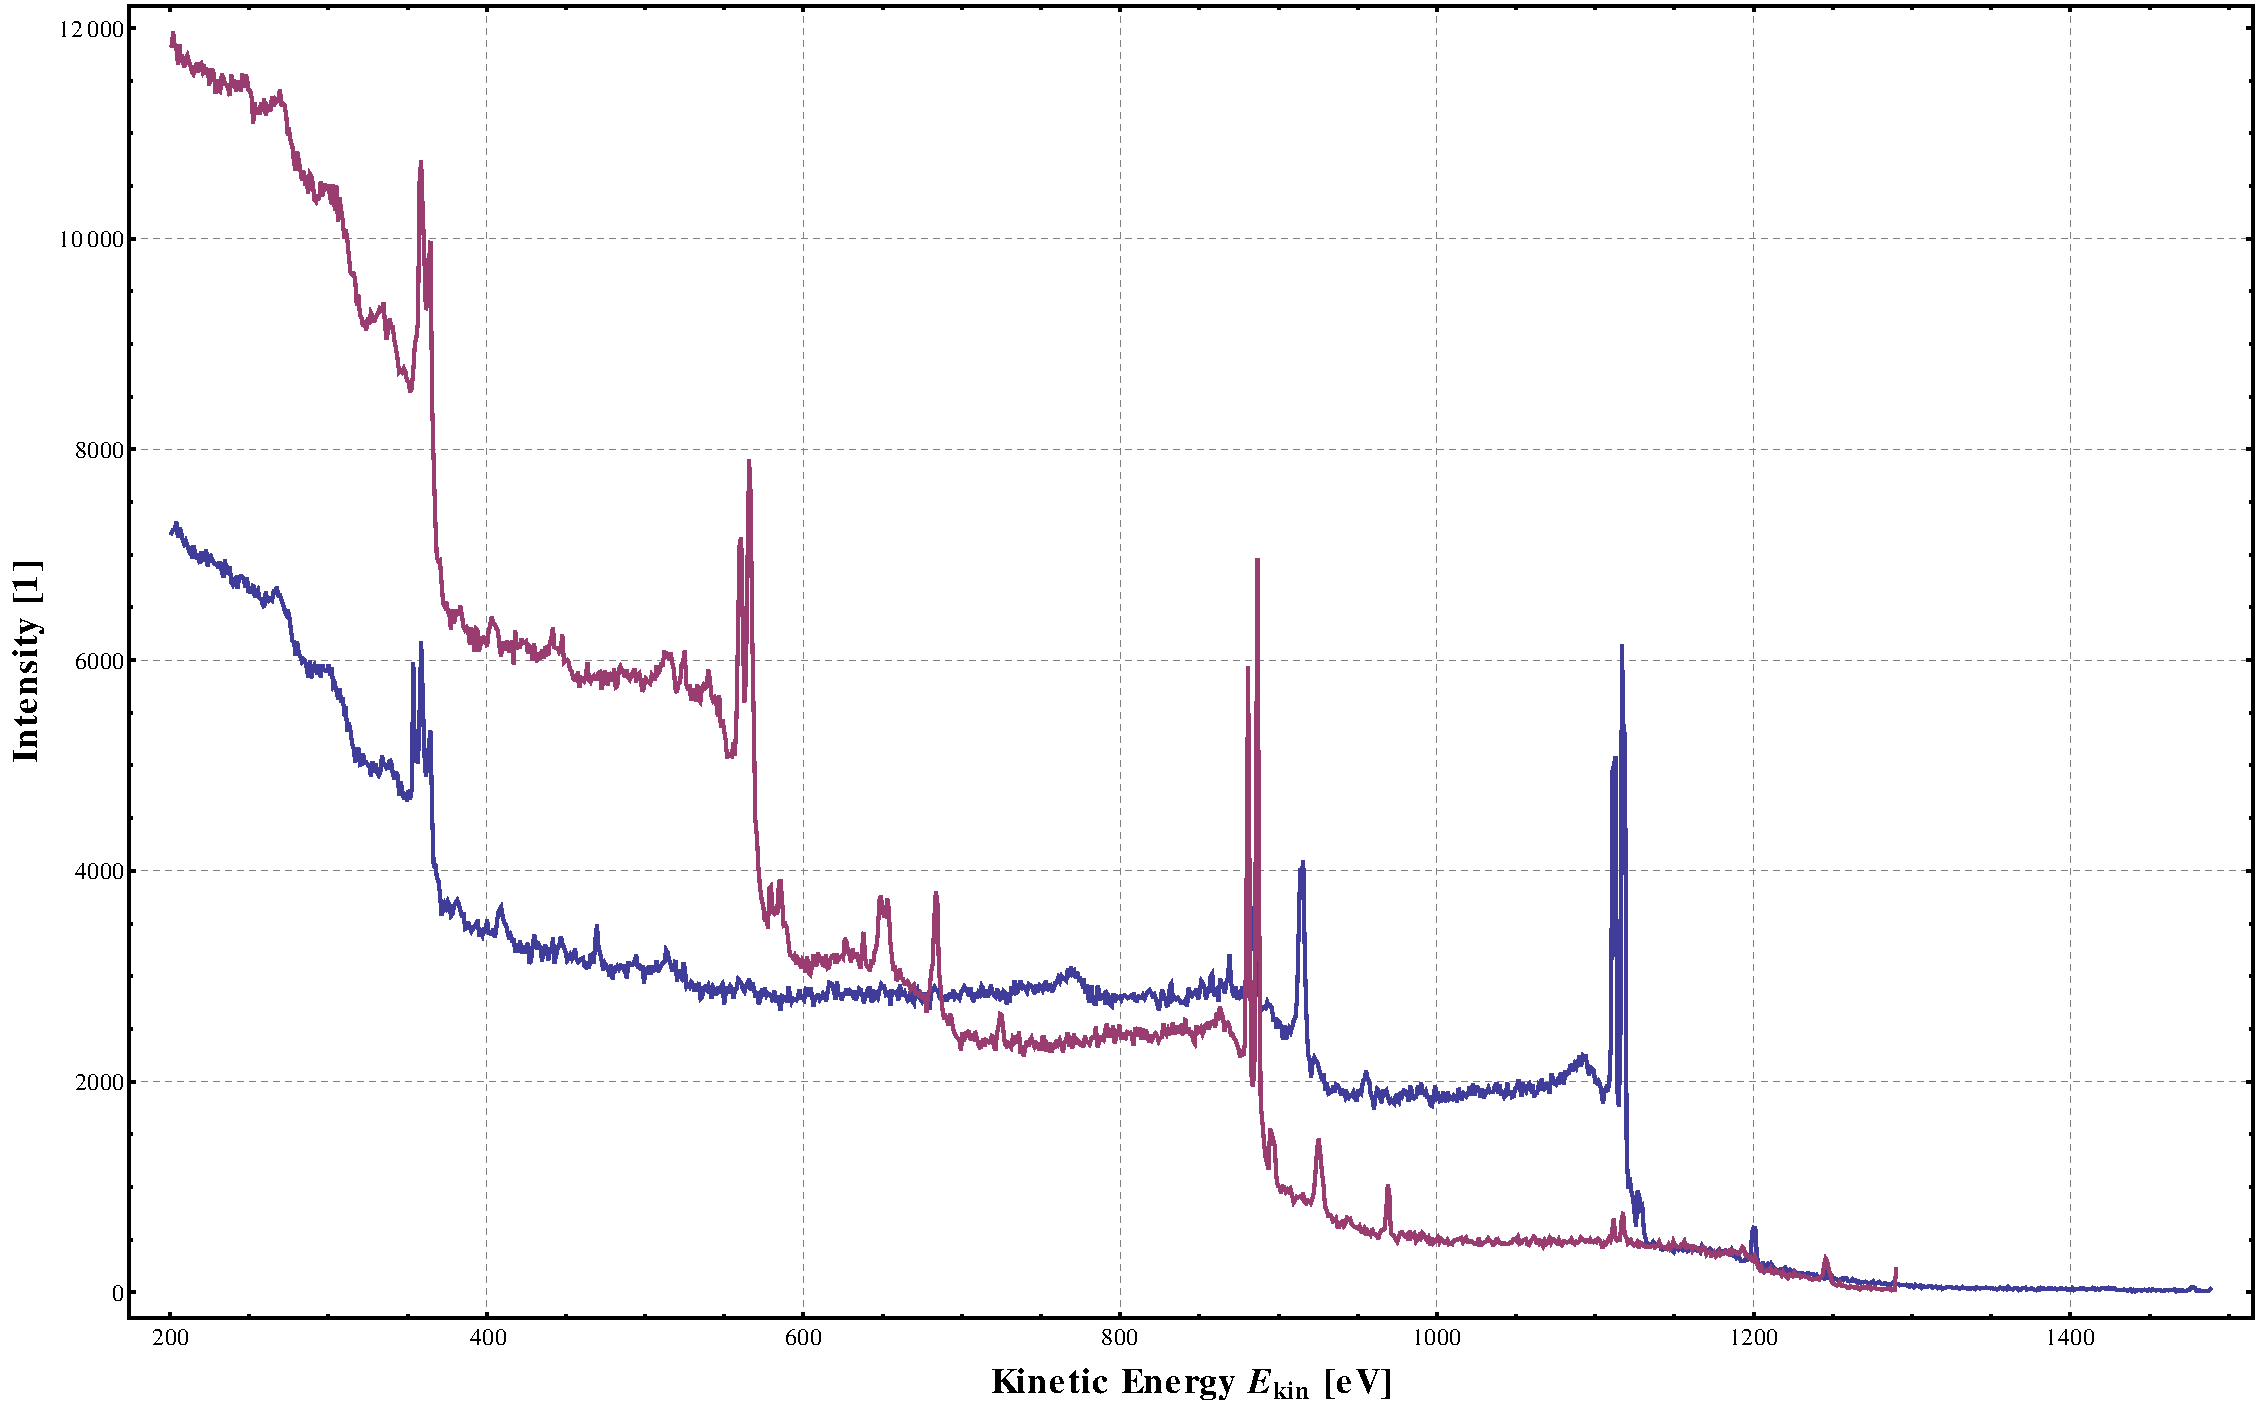
\includegraphics[scale=0.3]{img/silver_kinetic_both}
\caption{Kinetic energy spectra of the silver sample taken with both anodes \label{fig:ag_kinetic}}
\end{figure}

\begin{figure}
\centering
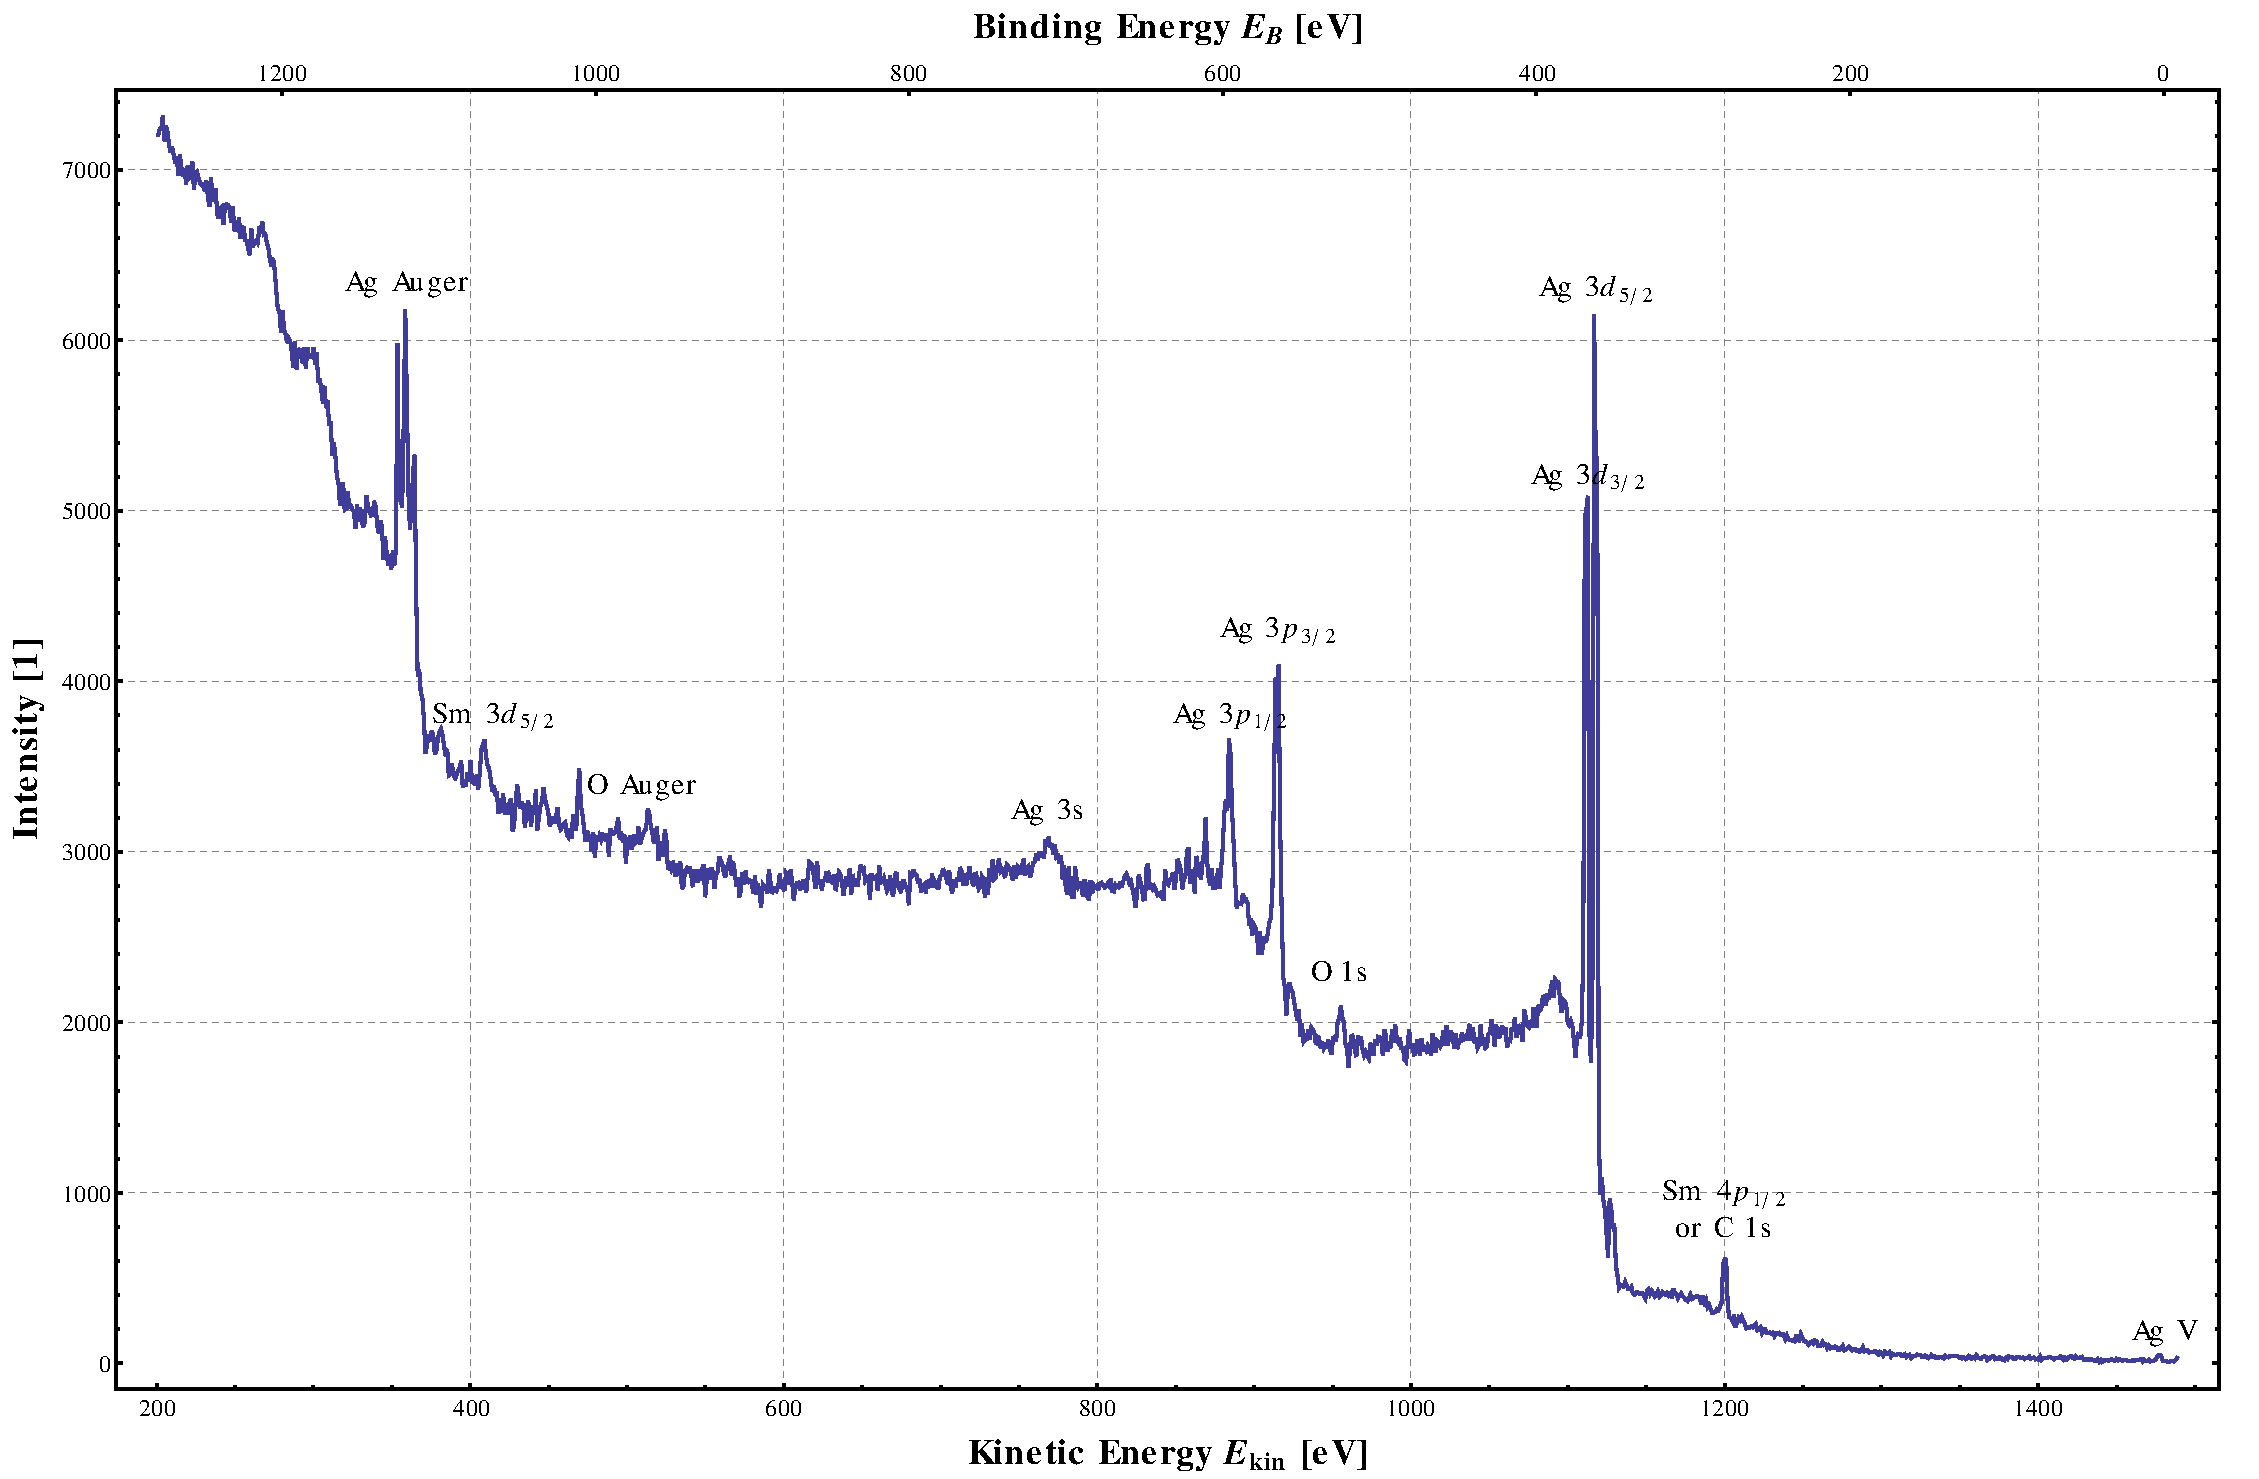
\includegraphics[scale=0.3]{img/silver_binding_al}
\caption{Spectrum of silver sample taken with aluminium anode \label{fig:ag_al}}
\end{figure}

\begin{figure}
\centering
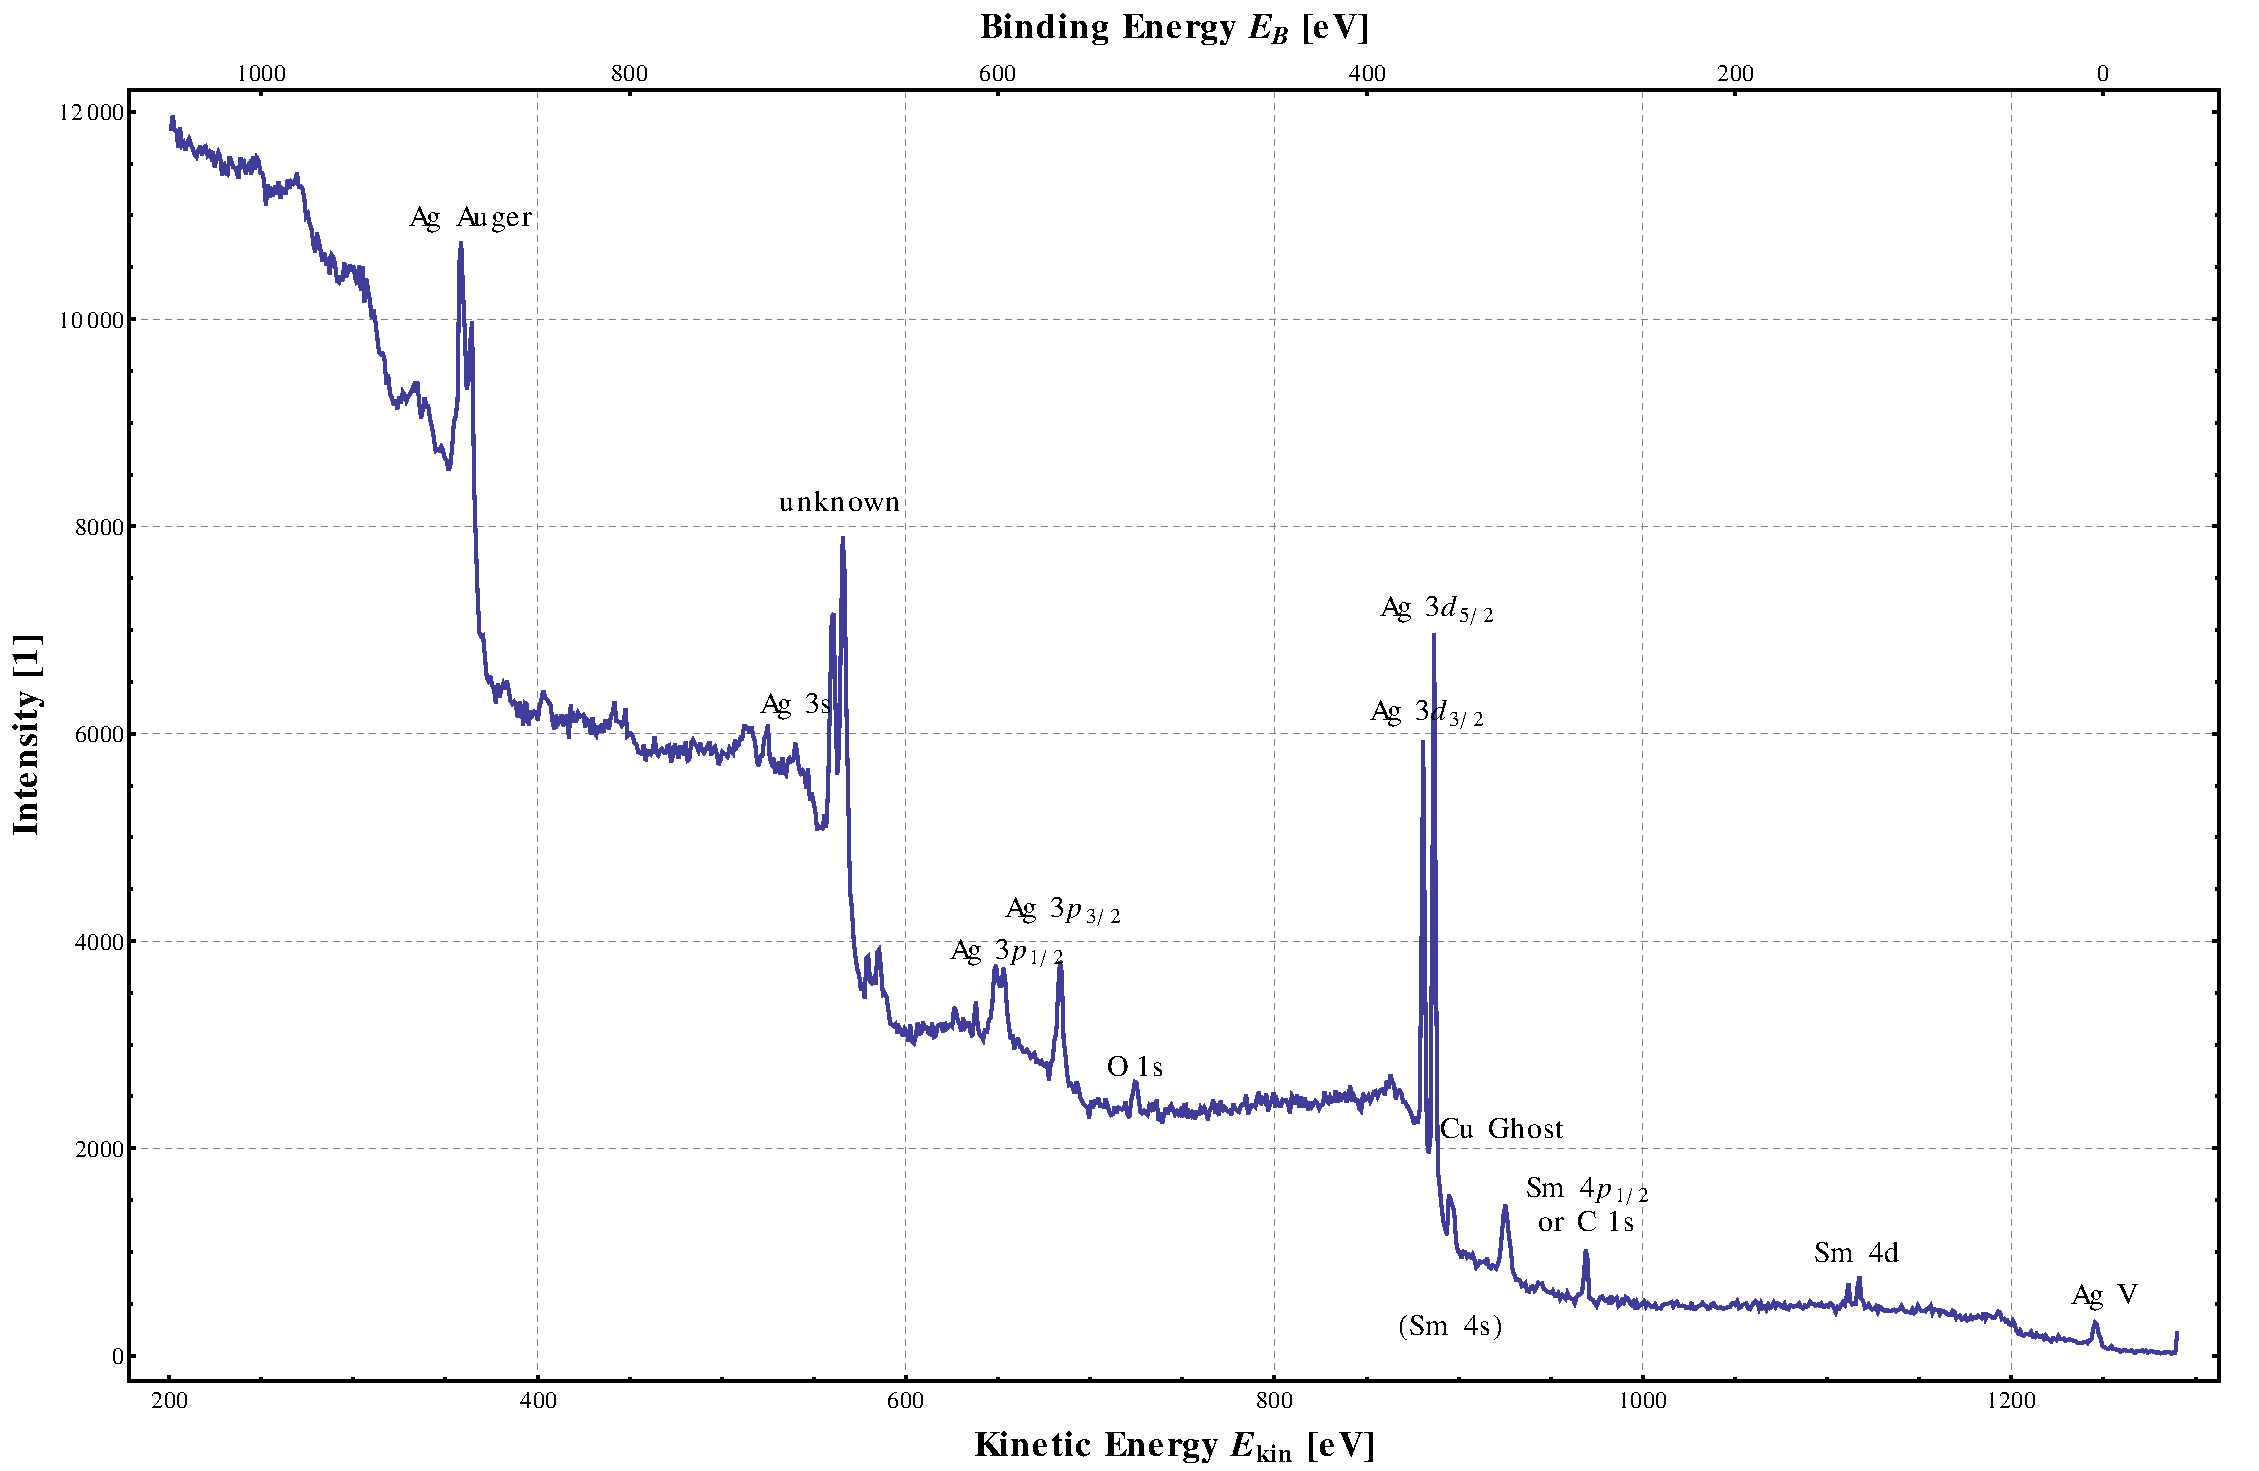
\includegraphics[scale=0.3]{img/silver_binding_mg}
\caption{Spectrum of silver sample taken with magnesium anode \label{fig:ag_mg}}
\end{figure}


\begin{table}
\begin{center}
\begin{tabular}{lcccc}
\toprule
Measured $E_{B}$ [eV]        & Identification & Theoretical$E_{B}$ [eV] & Abs. Dev. [eV] & Dev. [\%]\\
\midrule
\phantom{0}278.0 $\pm$ 1.5   & Sm $4p_{1/2}$  & 283                     & $-5.0$         & $-1.8$\\
\phantom{0}278.0 $\pm$ 1.5   & C $1s$         & 285                     & $-7.0$         & $-2.5$\\
\phantom{0}360.5 $\pm$ 1.5   & Ag $3d_{5/2}$  & 368                     & $-7.5$         & $-2.0$\\
\phantom{0}366.0 $\pm$ 1.5   & Ag $3d_{3/2}$  & 374                     & $-8.0$         & $-2.1$\\
\phantom{0}523.0 $\pm$ 2.3   & O $1s$         & 531                     & $-8.0$         & $-1.5$\\
\phantom{0}563.5 $\pm$ 1.5   & Ag $3p_{3/2}$  & 573                     & $-9.5$         & $-1.7$\\
\phantom{0}594.5 $\pm$ 1.9   & Ag $3p_{1/2}$  & 604                     & $-9.5$         & $-1.6$\\
\phantom{0}710.0 $\pm$ 5.1   & Ag $3s$        & 712                     & $-2.0$         & $-0.3$\\
\phantom{0}969.0 $\pm$ 5.1   & O Auger        & 978                     & $-9.0$         & $-0.9$\\
1069.0 $\pm$ 2.3             & Sm $3d_{5/2}$  & 1081                    & $-12.0$        & $-1.1$\\
1113.0 $\pm$ 1.5             & Ag Auger       & 1129                    & $-16.0$        & $-1.4$\\
\bottomrule
\end{tabular}
\end{center}
\par
\caption{Binding energies obtained from silver spectrum taken with aluminium anode~\ref{fig:ag_al} \label{tab:ag_al_ident}}
\end{table}

\begin{table}
\begin{center}
\begin{tabular}{lcccc}
\toprule
Measured $E_{B}$ [eV]        & Identification & Theoretical$E_{B}$ [eV] & Abs. Dev. [eV] & Dev. [\%]\\
\midrule
130.5 $\pm$ 1.5              & Sm $4d$        & 129                     & $1.5$          & $1.2$ \\
136.5 $\pm$ 1.5              & unknown        &                         &                &       \\
279.0 $\pm$ 1.5              & Sm $4p_{1/2}$  & 283                     & $-4.0$         & $-1.4$\\
279.0 $\pm$ 1.5              & C $1s$         & 285                     & $-6.0$         & $-2.1$\\
325.0 $\pm$ 1.9              & Cu Ghost       &                         &                &       \\
353.0 $\pm$ 1.5              & (Sm 4s)        & 349                     & $4.0$          & $1.1$ \\
361.5 $\pm$ 1.5              & Ag $3d_{5/2}$  & 368                     & $-6.5$         & $-1.8$\\
367.5 $\pm$ 1.5              & Ag $3d_{3/2}$  & 374                     & $-6.5$         & $-1.7$\\
523.5 $\pm$ 1.5              & O $1s$         & 525                     & $-1.5$         & $-0.3$\\
564.5 $\pm$ 1.9              & Ag $3p_{3/2}$  & 573                     & $-8.5$         & $-1.5$\\
595.0 $\pm$ 1.5              & Ag $3p_{1/2}$  & 604                     & $-9.0$         & $-1.5$\\
599.5 $\pm$ 1.5              & Ag $3p_{1/2}$  & 604                     & $-4.5$         & $-0.7$\\
682.5 $\pm$ 1.5              & unknown        &                         &                &       \\
688.0 $\pm$ 1.5              & unknown        &                         &                &       \\
708.0 $\pm$ 2.3              & Ag $3s$        & 719                     & $-11.0$        & $-1.5$\\
884.0 $\pm$ 1.9              & Ag Auger       & 896                     & $-12.0$        & $-1.3$\\
\bottomrule
\end{tabular}
\end{center}
\par
\caption{Binding energies obtained from silver spectrum taken with magnesium anode~\ref{fig:ag_mg} \label{tab:ag_mg_ident}}
\end{table}

\subsection{Samarium}

\begin{figure}
\centering
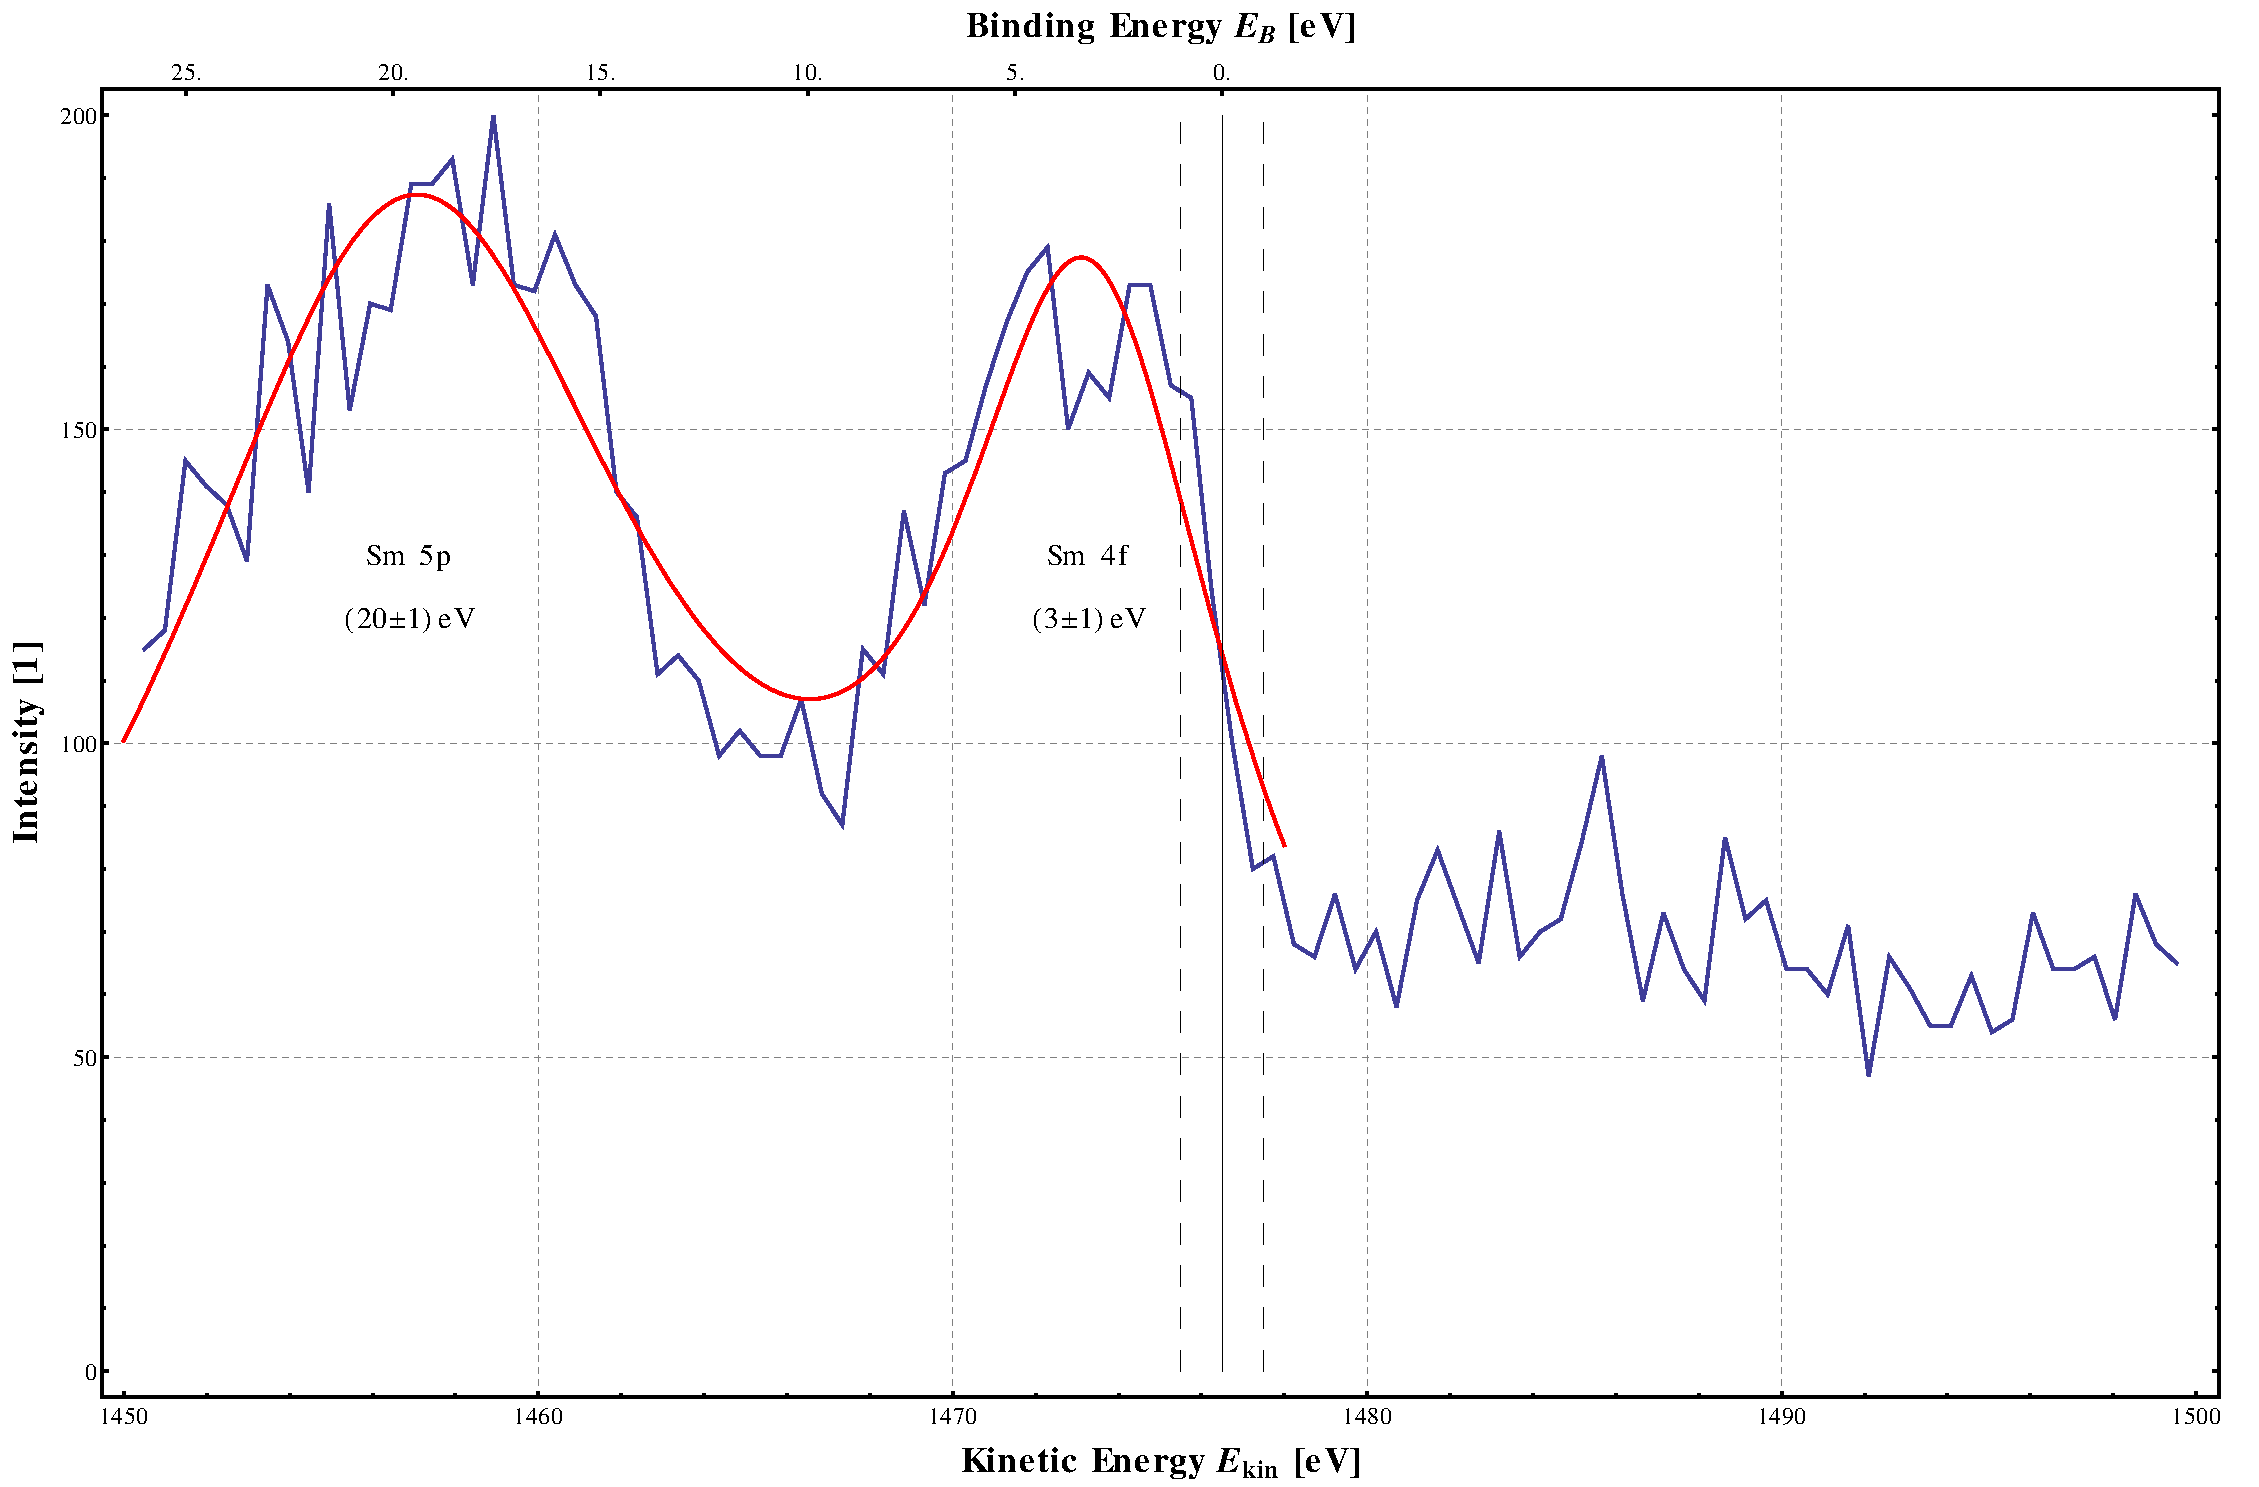
\includegraphics[scale=0.3]{img/samarium_fermiedge_al}
\caption{Spectrum of the samarium Fermi edge and 4f and 5p state \label{fig:sm_fermi}}
\end{figure}

\begin{figure}
\centering
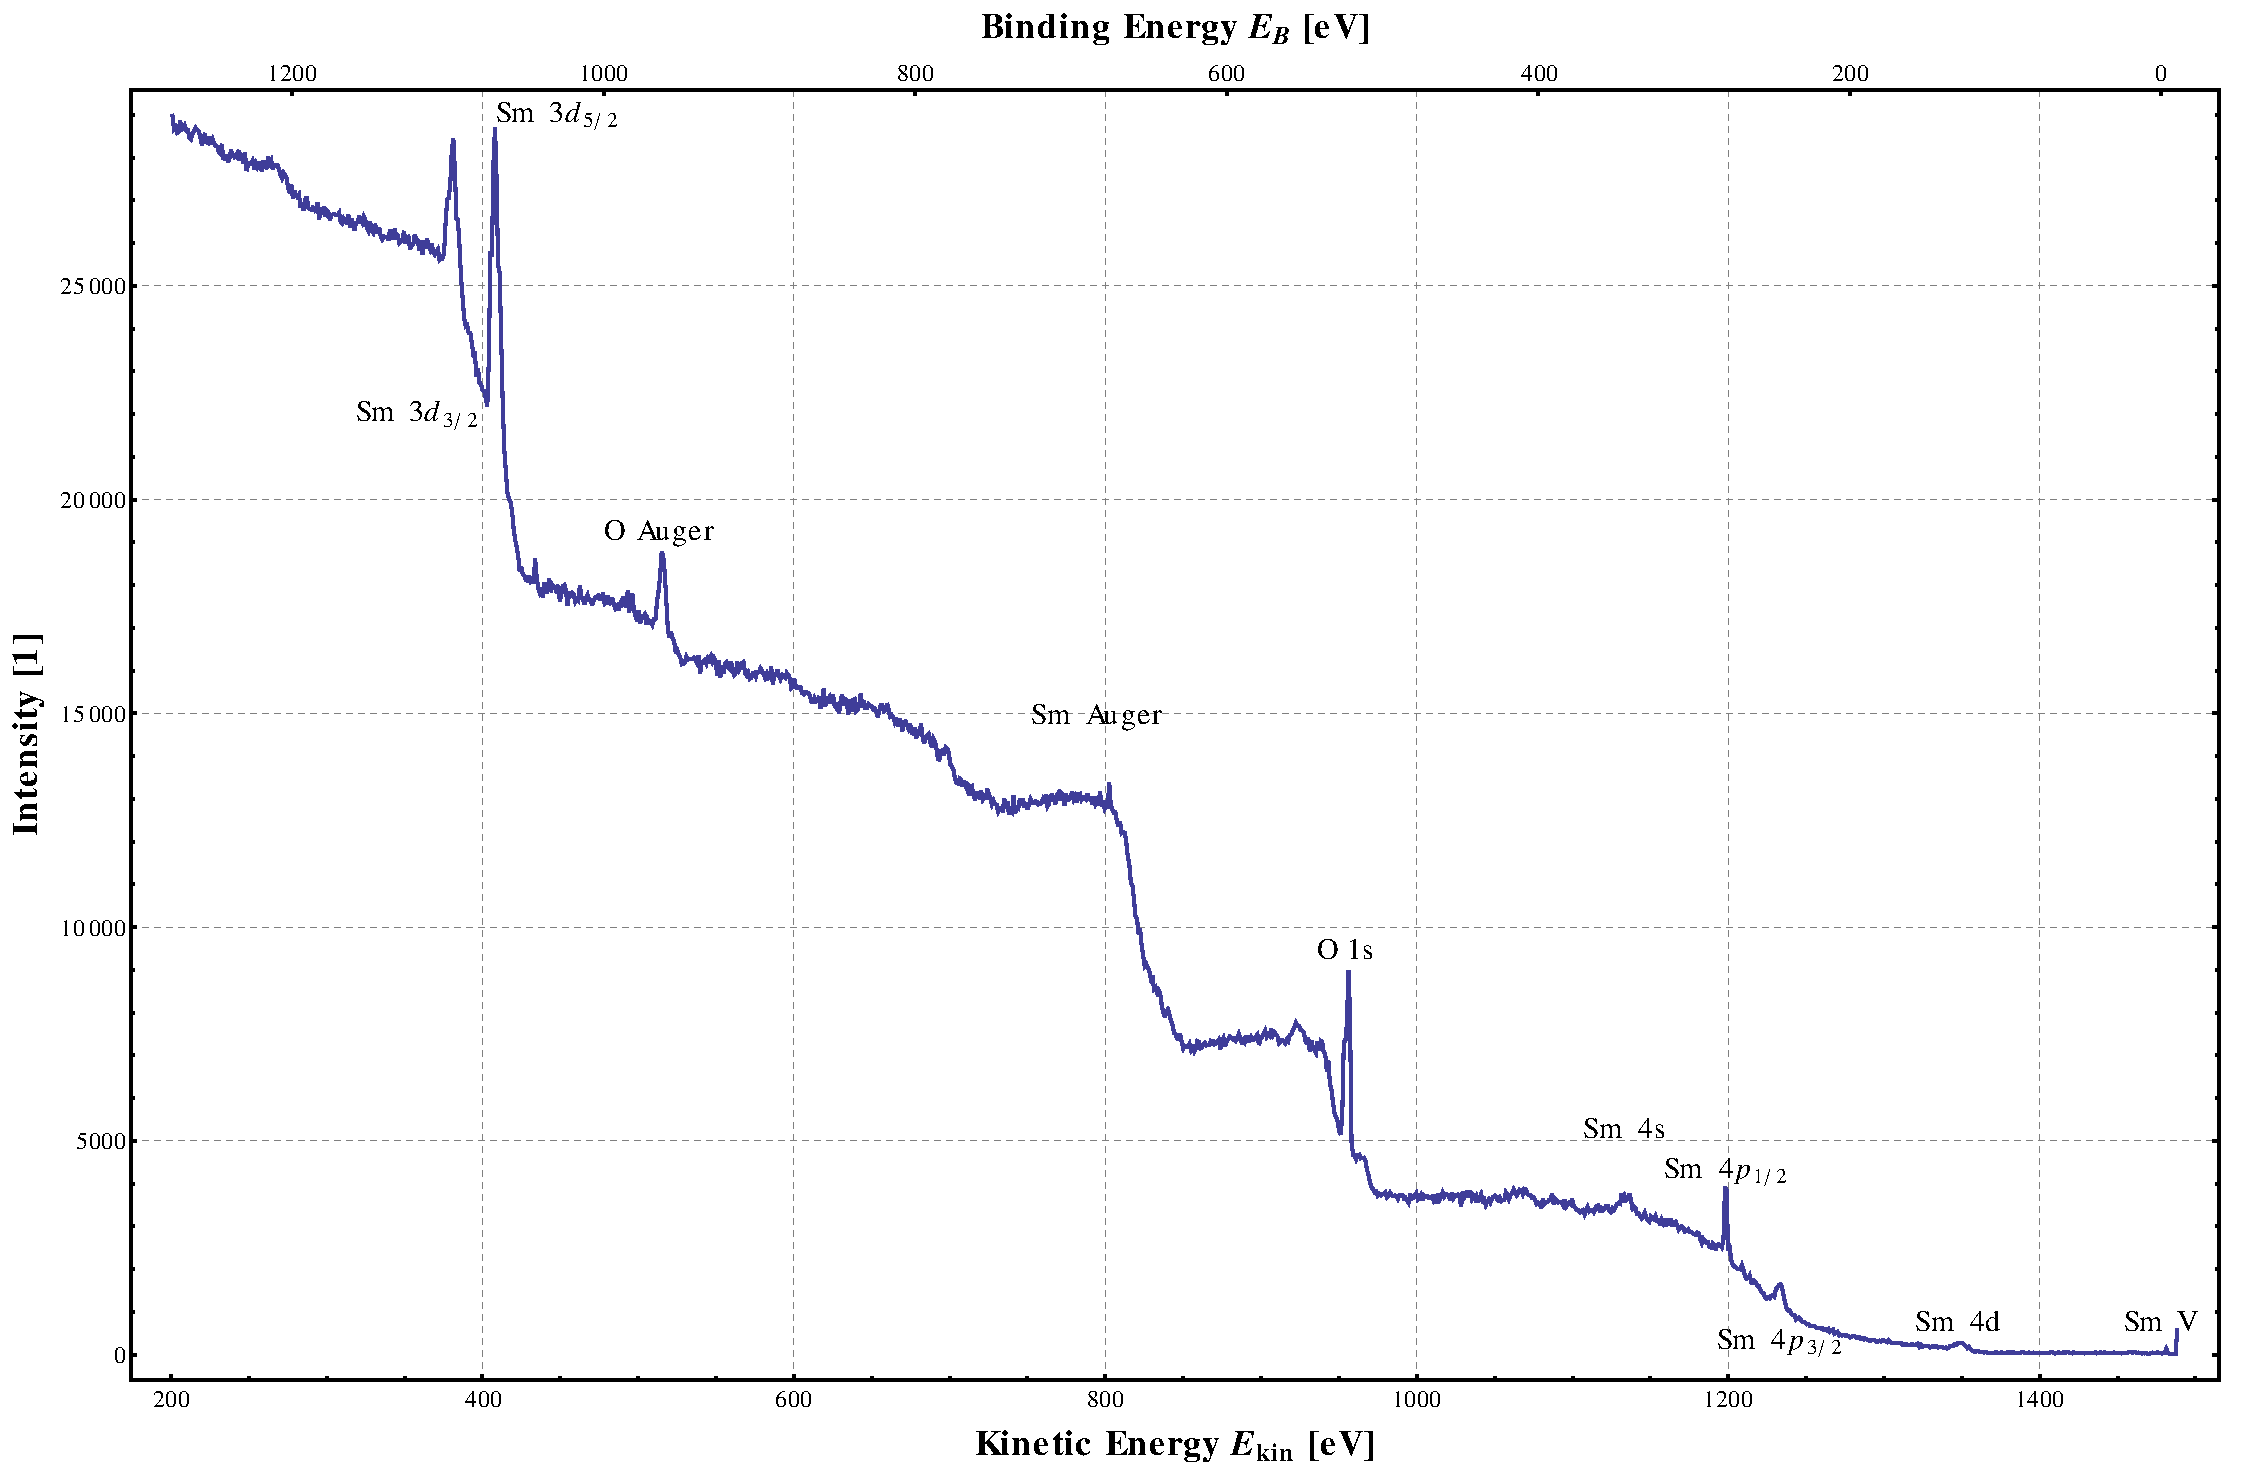
\includegraphics[scale=0.3]{img/samarium_binding_al}
\caption{Spectrum of samarium sample taken with aluminium anode \label{fig:sm_al}}
\end{figure}

\begin{figure}
\centering
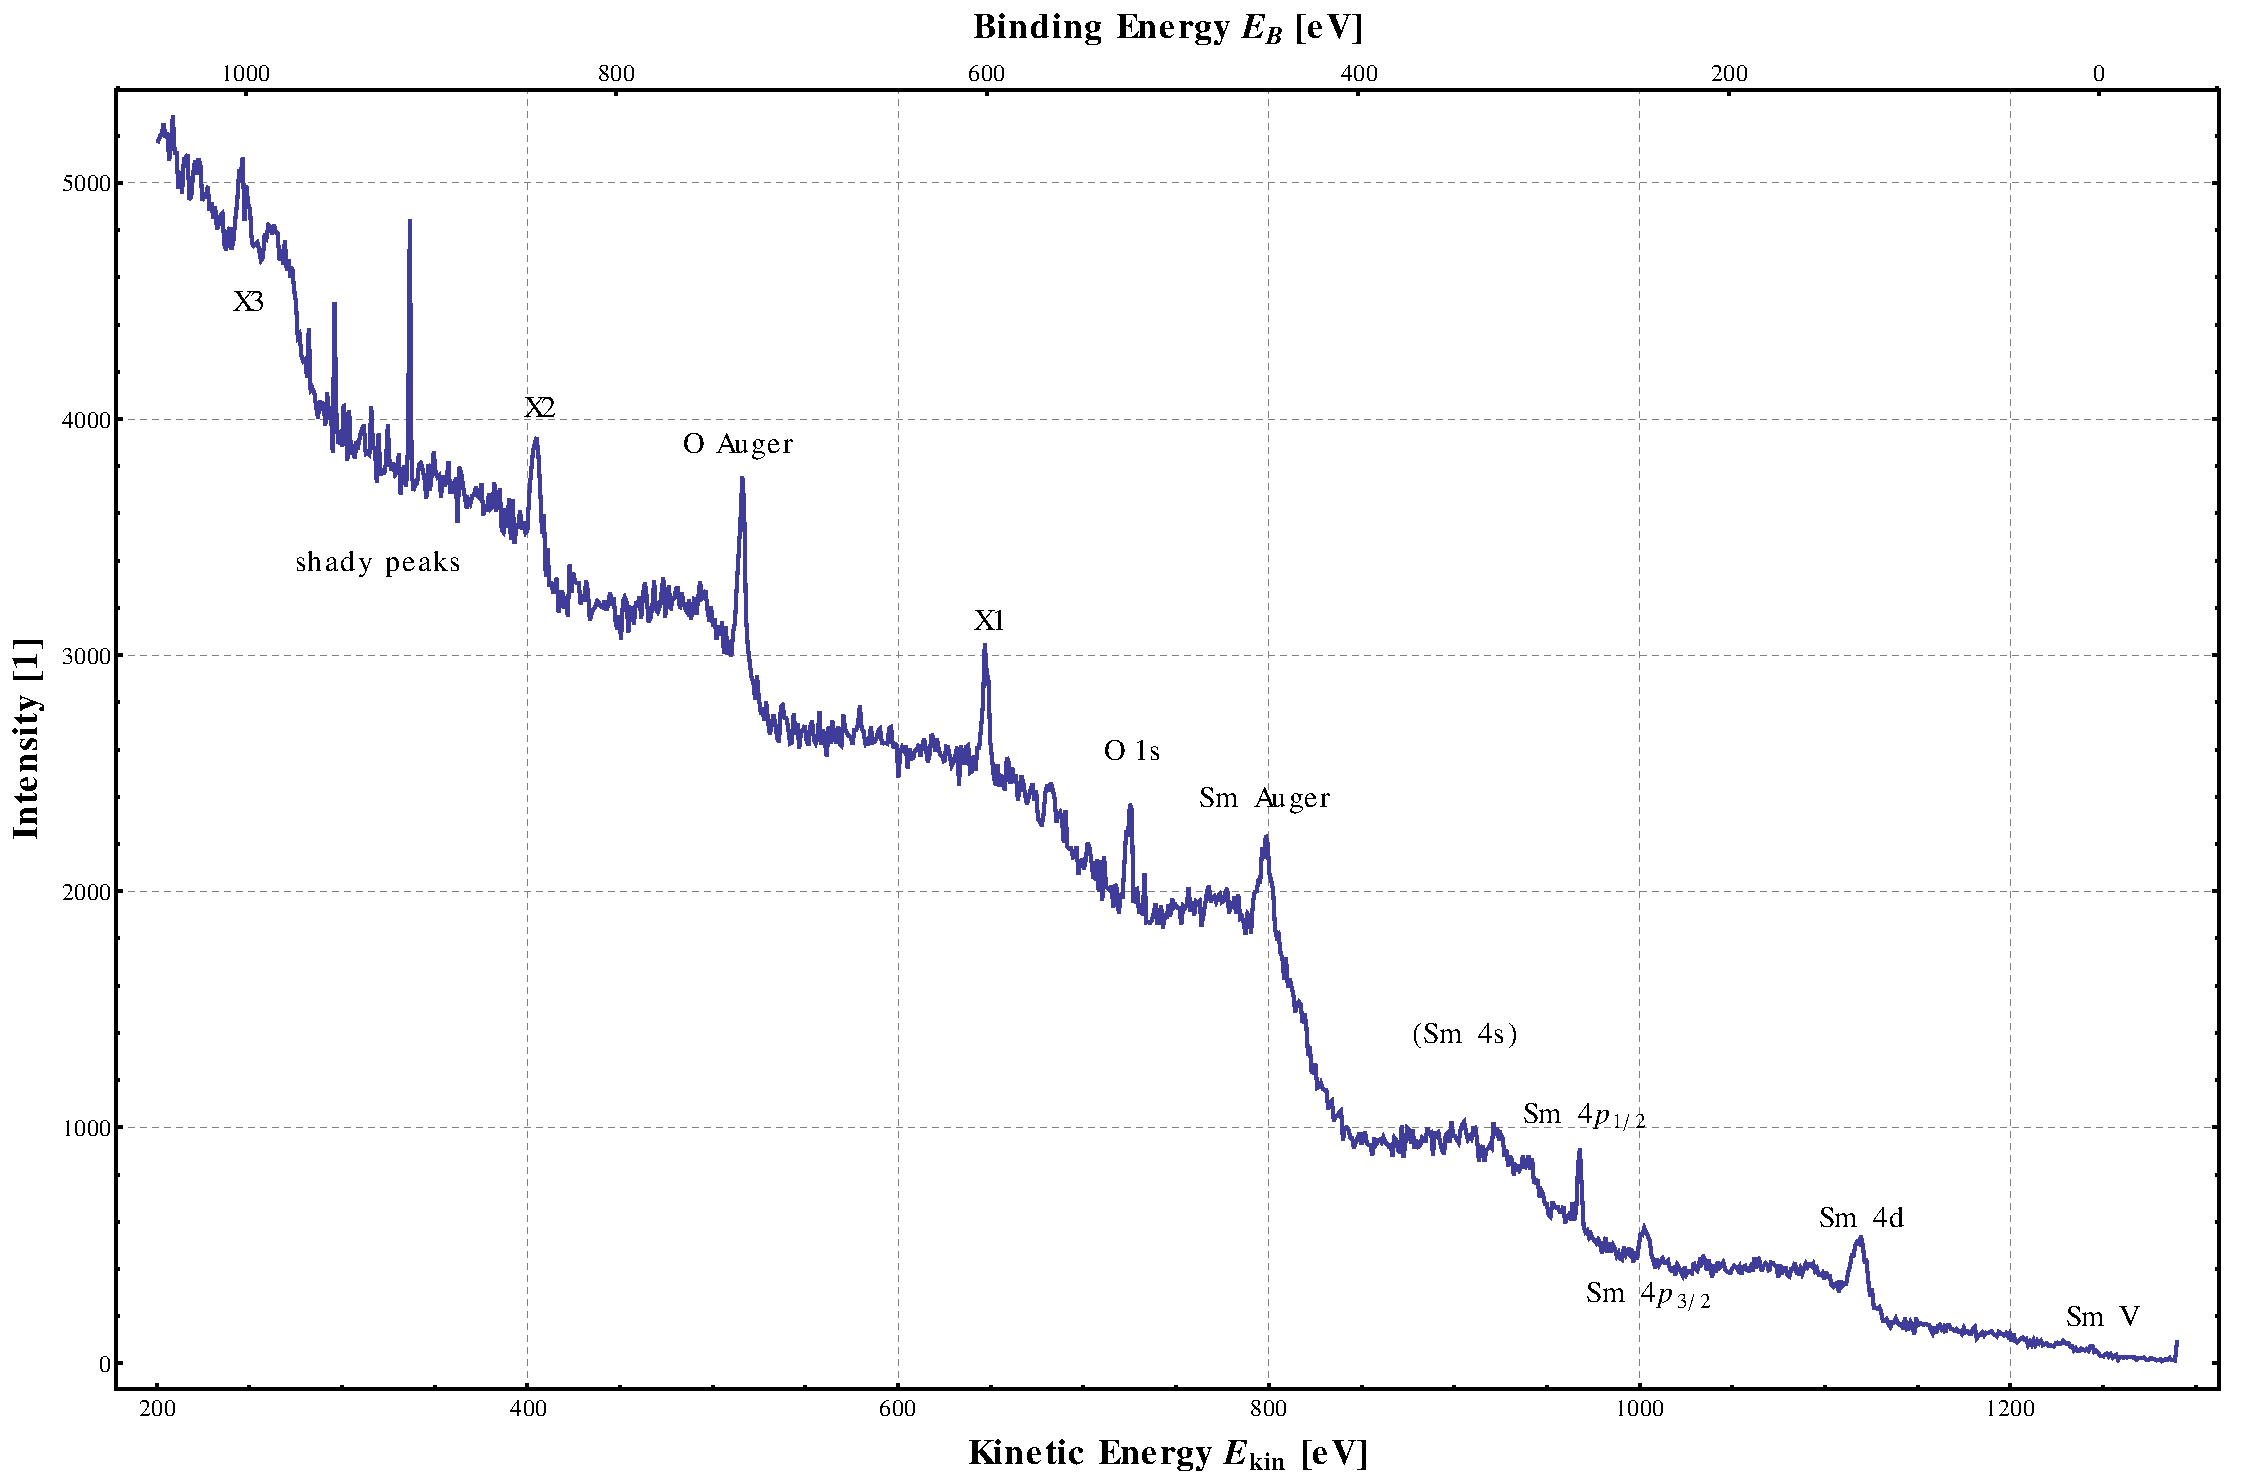
\includegraphics[scale=0.3]{img/samarium_binding_mg}
\caption{Spectrum of samarium sample taken with magnesium anode \label{fig:sm_mg}}
\end{figure}


\begin{table}
\begin{center}
\begin{tabular}{lcccc}
\toprule
Measured $E_{B}$ [eV]      & Identification & Theoretical$E_{B}$ [eV] & Abs. Dev. [eV] & Dev. [\%]\\
\midrule
\phantom{0}128.0 $\pm$ 1.5 & Sm $4d$        & 129                     & $-1.0$         & $-0.8$\\
\phantom{0}243.5 $\pm$ 2.3 & Sm $4p_{3/2}$  & 250                     & $-6.5$         & $-2.6$\\
\phantom{0}278.0 $\pm$ 1.5 & Sm $4p_{1/2}$  & 283                     & $-5.0$         & $-1.8$\\
\phantom{0}343.0 $\pm$ 2.3 & Sm $4s$        & 349                     & $-6.0$         & $-1.7$\\
\phantom{0}521.5 $\pm$ 1.9 & O $1s$         & 531                     & $-9.5$         & $-1.8$\\
\phantom{0}677.5 $\pm$ 5.1 & Sm Auger       & 682                     & $-4.5$         & $-0.7$\\
\phantom{0}961.0 $\pm$ 1.5 & O Auger        & 978                     & $-17.0$        & $-1.7$\\
1068.5 $\pm$ 1.9           & Sm $3d_{5/2}$  & 1081                    & $-12.5$        & $-1.2$\\
1095.5 $\pm$ 1.9           & Sm $3d_{3/2}$  & 1108                    & $-12.5$        & $-1.1$\\
\bottomrule
\end{tabular}
\end{center}
\par
\caption{Binding energies obtained from samarium spectrum taken with aluminium anode~\ref{fig:sm_al} \label{tab:sm_al_ident}}
\end{table}

\begin{table}
\begin{center}
\begin{tabular}{lcccc}
\toprule
Measured $E_{B}$ [eV]      & Identification & Theoretical$E_{B}$ [eV] & Abs. Dev. [eV] & Dev. [\%]\\
\midrule
\phantom{0}129.0 $\pm$ 2.3 & Sm $4d$        & 129                     & $0.0$          & $0.0$ \\
\phantom{0}245.0 $\pm$ 1.9 & Sm $4p_{3/2}$  & 250                     & $-5.0$         & $-2.0$\\
\phantom{0}280.0 $\pm$ 1.5 & Sm $4p_{1/2}$  & 283                     & $-3.0$         & $-1.1$\\
\phantom{0}342.0 $\pm$ 5.1 & Sm $4s$        & 349                     & $-7.0$         & $-2.0$\\
\phantom{0}449.5 $\pm$ 2.3 & Sm Auger       & 449                     & $0.5$          & $0.1$ \\
\phantom{0}523.0 $\pm$ 1.9 & O $1s$         & 531                     & $-8.0$         & $-1.5$\\
\phantom{0}600.0 $\pm$ 1.5 & X1             &                         &                &       \\
\phantom{0}731.5 $\pm$ 1.9 & O Auger        & 745                     & $-13.5$        & $-1.8$\\
\phantom{0}843.0 $\pm$ 2.3 & X2             &                         &                &       \\
1000.0 $\pm$ 1.5           & X3             &                         &                &       \\
\bottomrule
\end{tabular}
\end{center}
\par
\caption{Binding energies obtained from samarium spectrum taken with magnesium anode~\ref{fig:sm_mg} \label{tab:sm_mg_ident}}
\end{table}

\subsection{Coin}

\begin{figure}
\centering
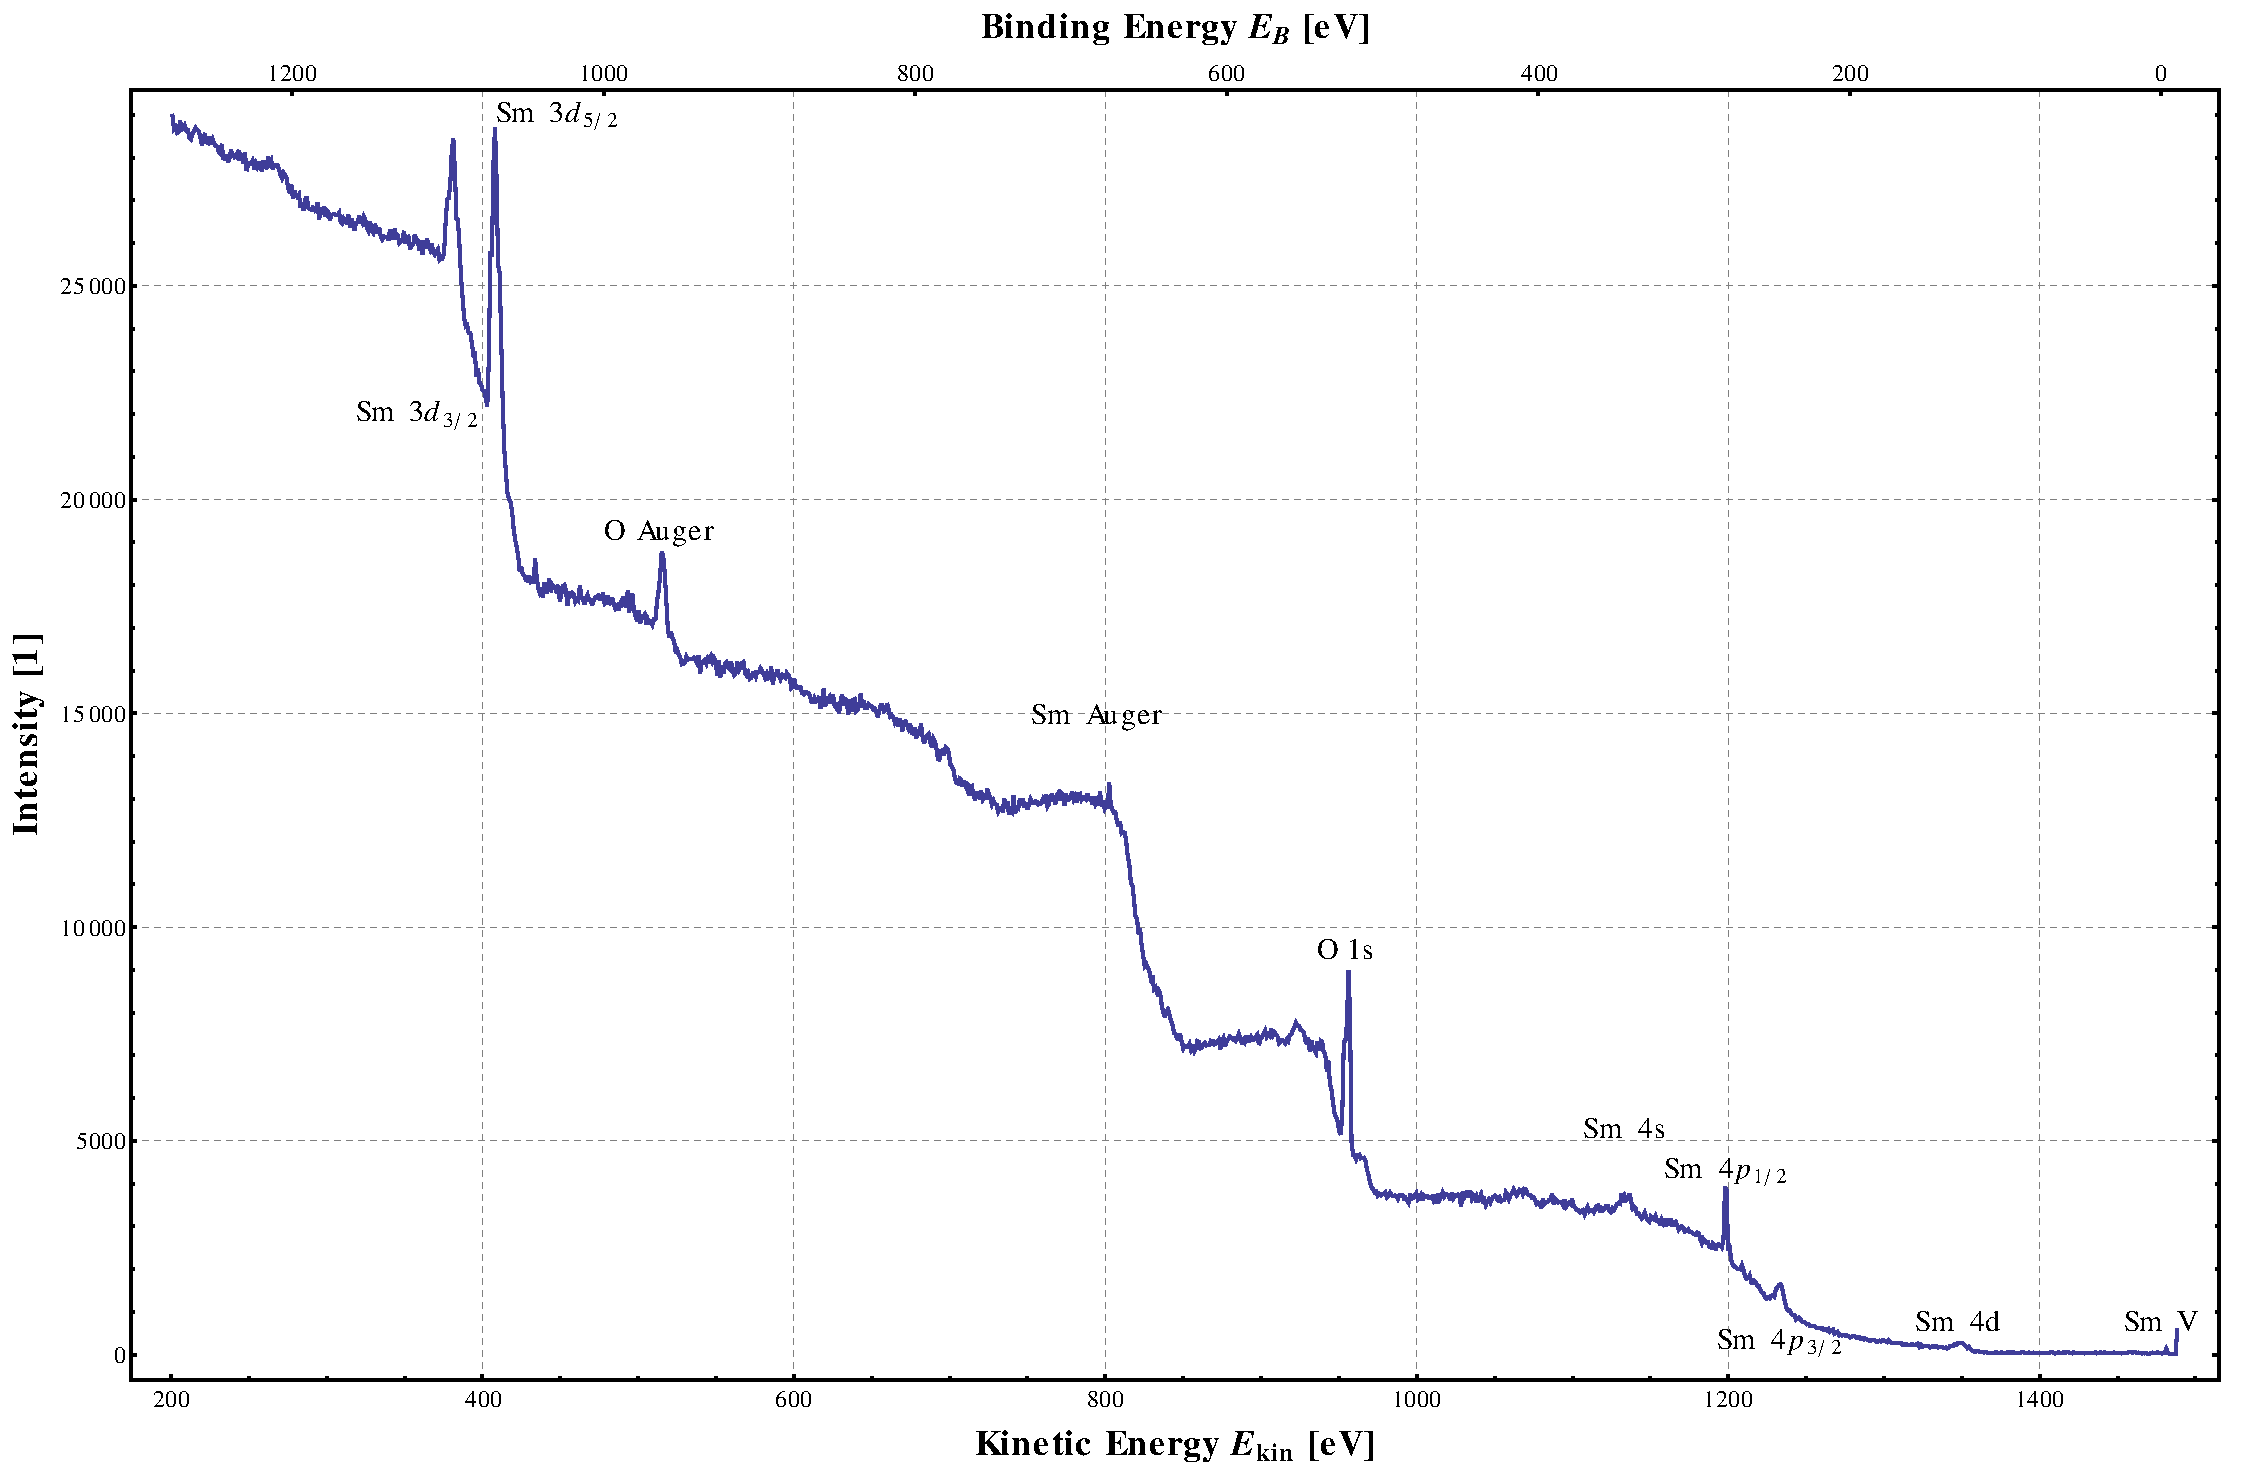
\includegraphics[scale=0.3]{img/samarium_binding_al}
\caption{Spectrum of the coin taken with aluminium anode \label{fig:coin_al}}
\end{figure}

\begin{figure}
\centering
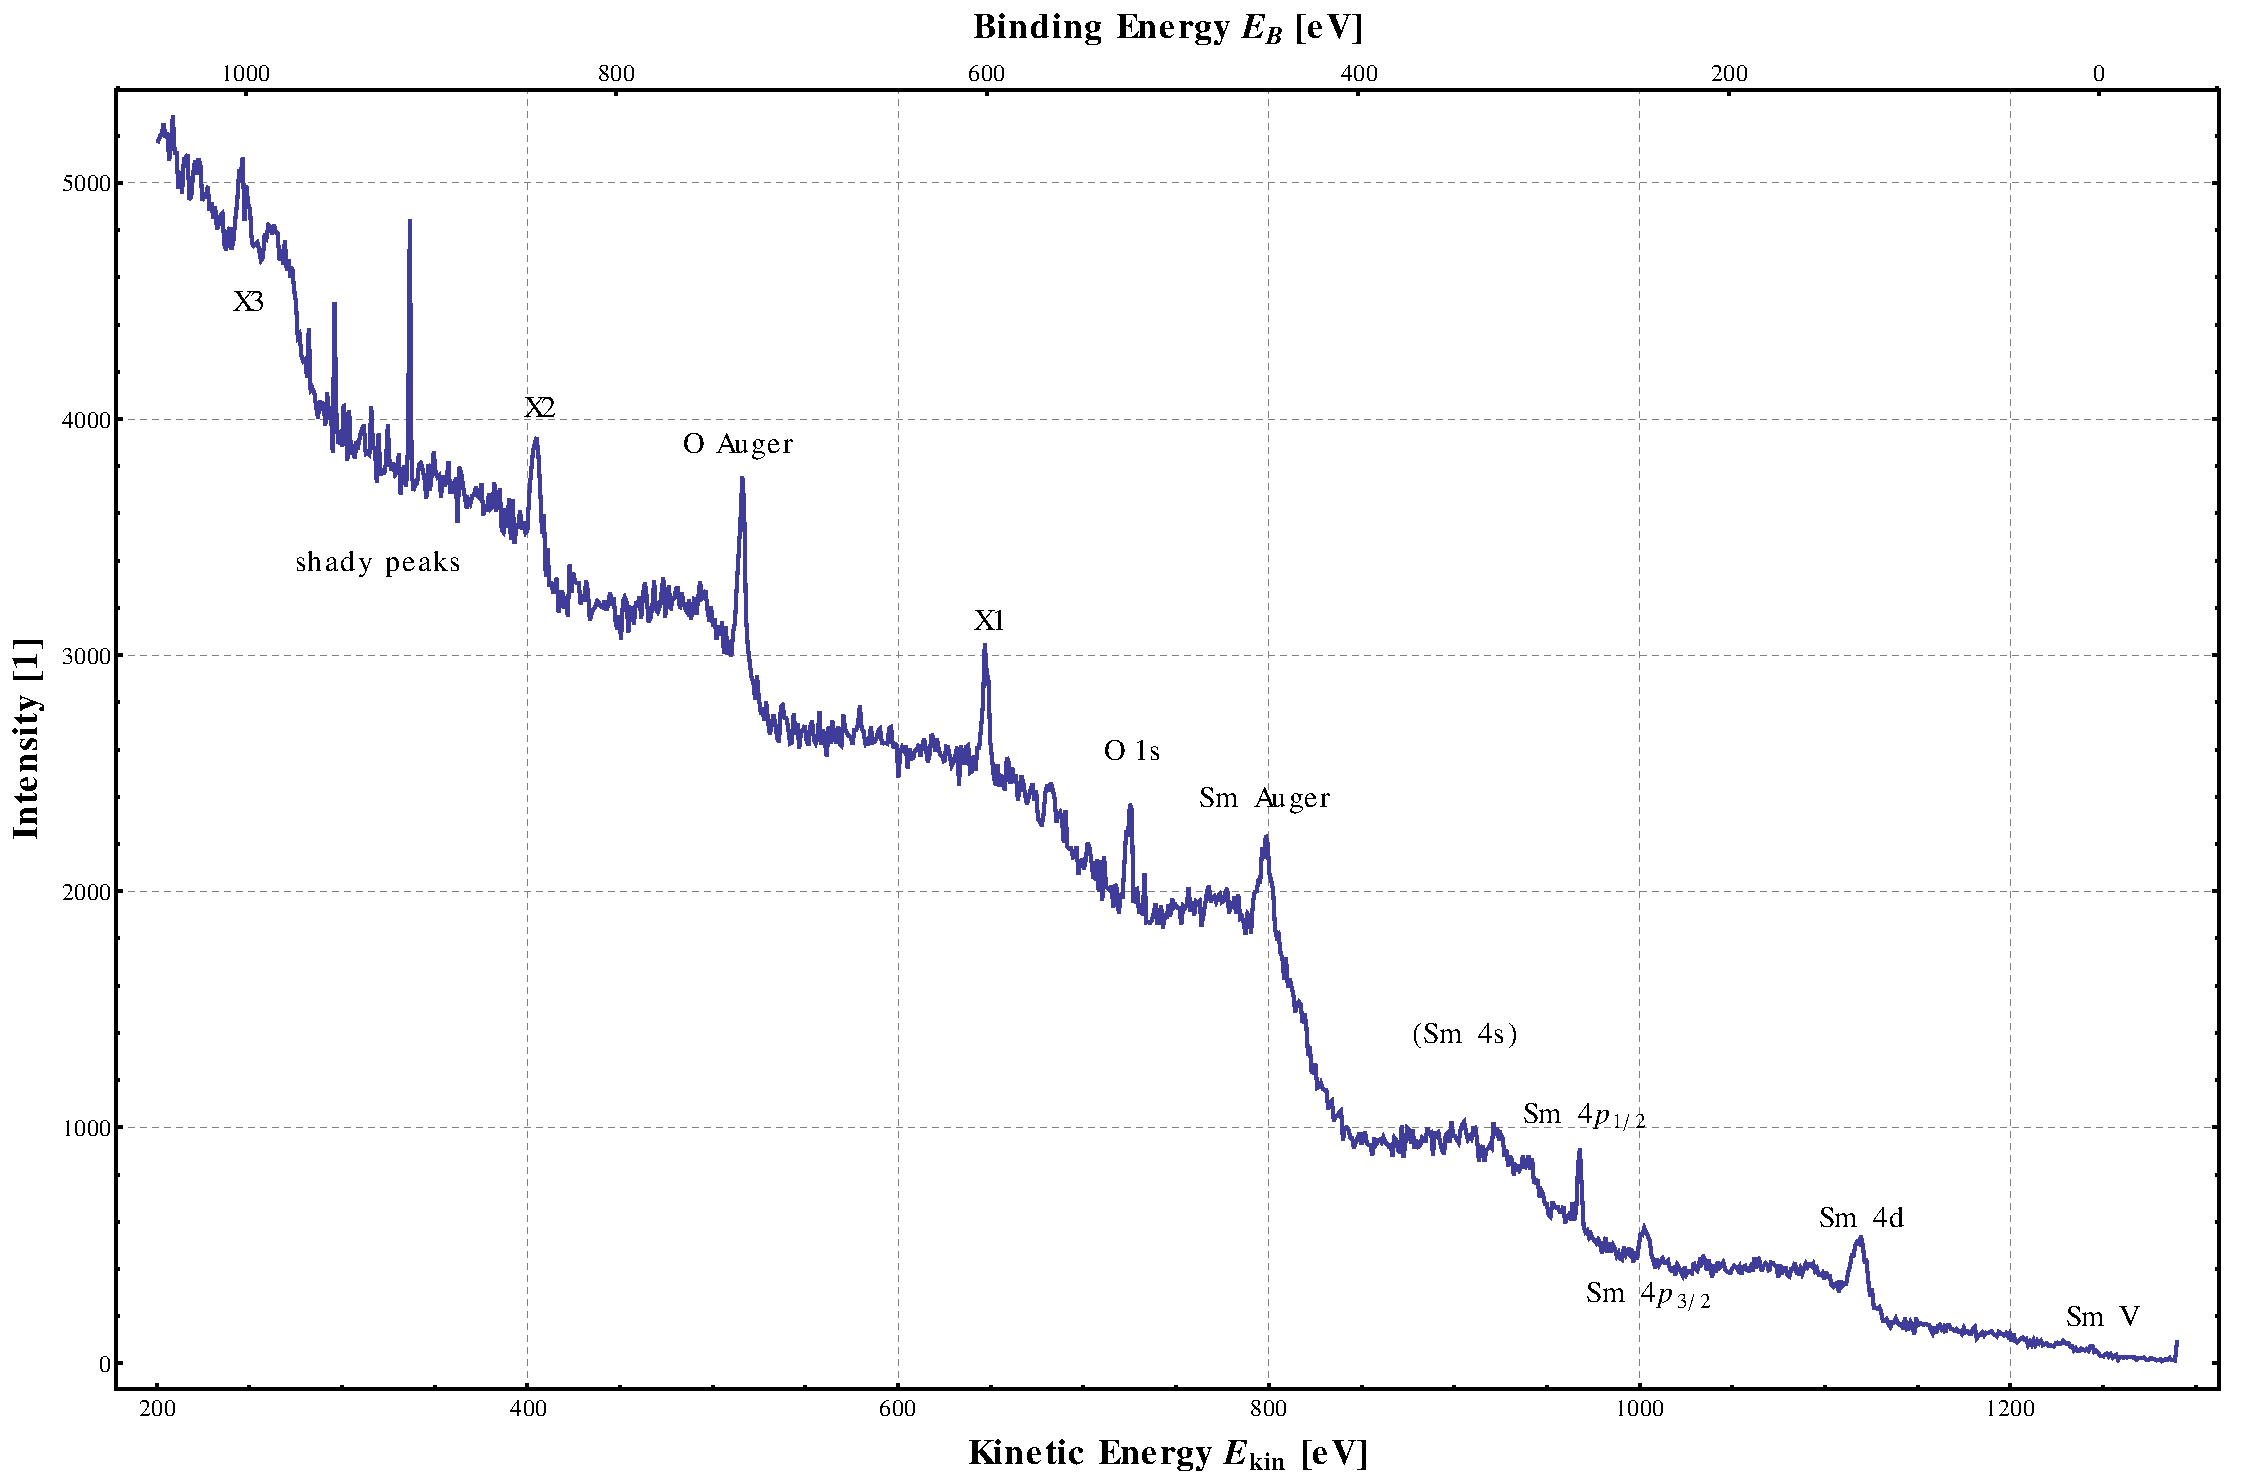
\includegraphics[scale=0.3]{img/samarium_binding_mg}
\caption{Spectrum of the coin taken with magnesium anode \label{fig:coin_mg}}
\end{figure}


\begin{table}
\begin{center}
\begin{tabular}{lcccc}
\toprule
Measured $E_{B}$ [eV]      & Identification & Theoretical$E_{B}$ [eV] & Abs. Dev. [eV] & Dev. [\%]\\
\midrule
\phantom{00}72.0 $\pm$ 2.3 & Cu $3p_{1/2}$  & 77                      & $-5.0$         & $-6.5$   \\
\phantom{0}129.0 $\pm$ 2.3 & Cu $3s$        & 123                     & $6.0$          & $4.9$    \\
\phantom{0}129.0 $\pm$ 2.3 & Sm $4d$        & 129                     & $0.0$          & $0.0$    \\
\phantom{0}245.0 $\pm$ 1.9 & Sm $4p_{3/2}$  & 250                     & $-5.0$         & $-2.0$   \\
\phantom{0}278.0 $\pm$ 1.5 & Sm $4p_{1/2}$  & 283                     & $-5.0$         & $-1.8$   \\
\phantom{0}278.0 $\pm$ 1.5 & C $1s$         & 285                     & $-7.0$         & $-2.5$   \\
\phantom{0}360.5 $\pm$ 1.5 & Ag $3d_{5/2}$  & 368                     & $-7.5$         & $-2.0$   \\
\phantom{0}366.5 $\pm$ 1.9 & Ag $3d_{3/2}$  & 374                     & $-7.5$         & $-2.0$   \\
\phantom{0}522.5 $\pm$ 1.9 & O $1s$         & 531                     & $-8.5$         & $-1.6$   \\
\phantom{0}562.5 $\pm$ 2.3 & Ag $3p_{3/2}$  & 573                     & $-10.5$        & $-1.8$   \\
\phantom{0}594.0 $\pm$ 2.3 & Ag $3p_{1/2}$  & 604                     & $-10.0$        & $-1.7$   \\
\phantom{0}674.5 $\pm$ 1.5 & Sm Auger       & 682                     & $-7.5$         & $-1.1$   \\
\phantom{0}710.0 $\pm$ 2.3 & Ag $3s$        & 719                     & $-9.0$         & $-1.3$   \\
\phantom{0}920.0 $\pm$ 1.5 & Cu $2p_{3/2}$  & 933                     & $-13.0$        & $-1.4$   \\
\phantom{0}939.5 $\pm$ 1.5 & Cu $2p_{1/2}$  & 953                     & $-13.5$        & $-1.4$   \\
\phantom{0}963.0 $\pm$ 2.3 & O Auger        & 965                     & $-2.0$         & $-0.2$   \\
1069.0 $\pm$ 2.3           & Sm $3d_{5/2}$  & 1081                    & $-12.0$        & $-1.1$   \\
1096.0 $\pm$ 2.3           & Sm $3d_{3/2}$  & 1108                    & $-12.0$        & $-1.1$   \\
1120.0 $\pm$ 5.1           & Ag Auger       & 1129                    & $-9.0$         & $-0.8$   \\
\bottomrule
\end{tabular}
\end{center}
\par
\caption{Binding energies obtained from the coin taken with aluminium anode~\ref{fig:coin_al} \label{tab:coin_al_ident}}
\end{table}

\begin{table}
\begin{center}
\begin{tabular}{lcccc}
\toprule
Measured $E_{B}$ [eV]      & Identification & Theoretical$E_{B}$ [eV] & Abs. Dev. [eV] & Dev. [\%]\\
\midrule
\phantom{00}74.0 $\pm$ 2.3 & Cu $3p_{1/2}$  & 77                      & $-3.0$         & $-3.9$\\
\phantom{0}130.0 $\pm$ 4.2 & Cu $3s$        & 123                     & $7.0$          & $5.7$ \\
\phantom{0}130.0 $\pm$ 4.2 & Sm $4d$        & 129                     & $1.0$          & $0.8$ \\
\phantom{0}279.0 $\pm$ 1.5 & Sm $4p_{1/2}$  & 283                     & $-4.0$         & $-1.4$\\
\phantom{0}279.0 $\pm$ 1.5 & C $1s$         & 285                     & $-6.0$         & $-2.1$\\
\phantom{0}450.0 $\pm$ 5.1 & Sm Auger       & 449                     & $1.0$          & $0.2$ \\
\phantom{0}523.5 $\pm$ 1.9 & O $1s$         & 531                     & $-7.5$         & $-1.4$\\
\phantom{0}600.0 $\pm$ 2.3 & (Ag 3p12)      & 604                     & $-4.0$         & $-0.7$\\
\phantom{0}733.0 $\pm$ 2.3 & O Auger        & 745                     & $-12.0$        & $-1.6$\\
\phantom{0}844.0 $\pm$ 2.3 & X1             &                         &                &       \\
1000.0 $\pm$ 1.5           & X2             &                         &                &       \\
\bottomrule
\end{tabular}
\end{center}
\par
\caption{Binding energies obtained from the coin spectrum taken with magnesium anode~\ref{fig:coin_mg} \label{tab:coin_mg_ident}}
\end{table}

\begin{figure}
\centering
\subfigure[ ]{
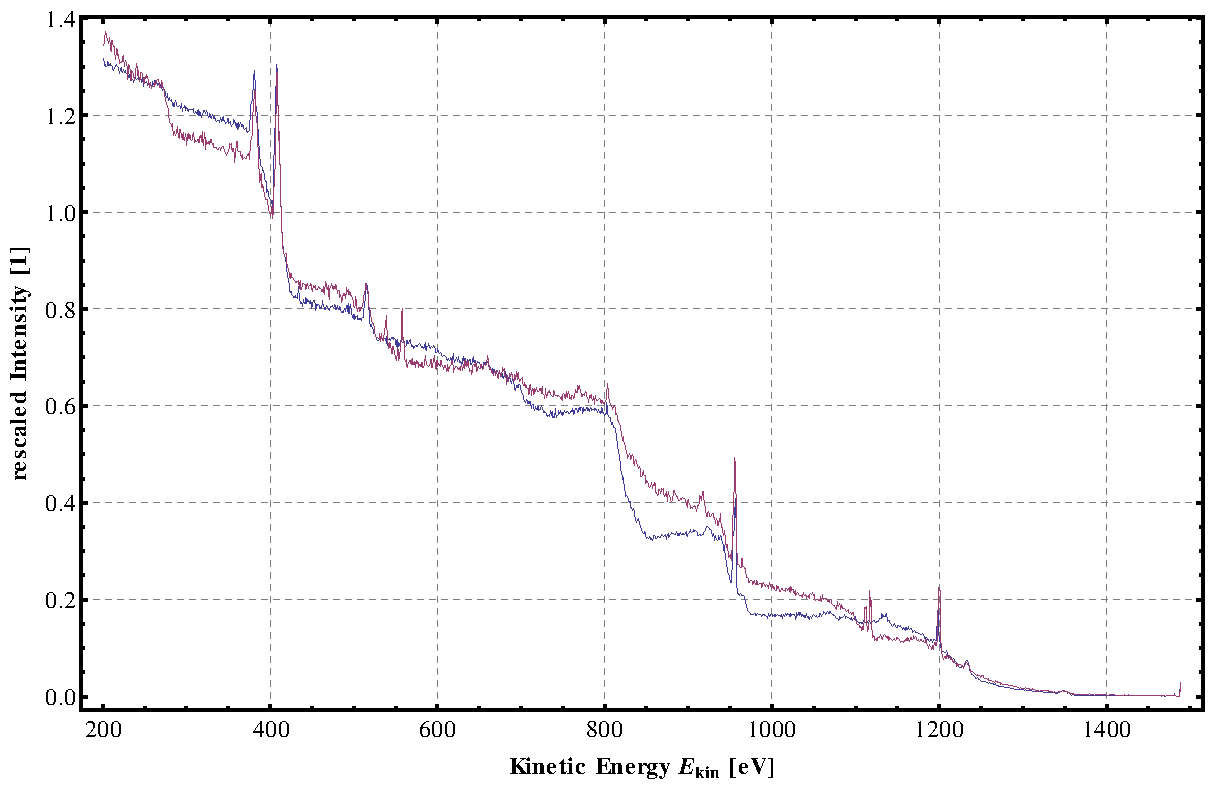
\includegraphics[scale=0.305]{img/samarium-coin_al}
\label{fig:smc_al}
}
\subfigure[ ]{
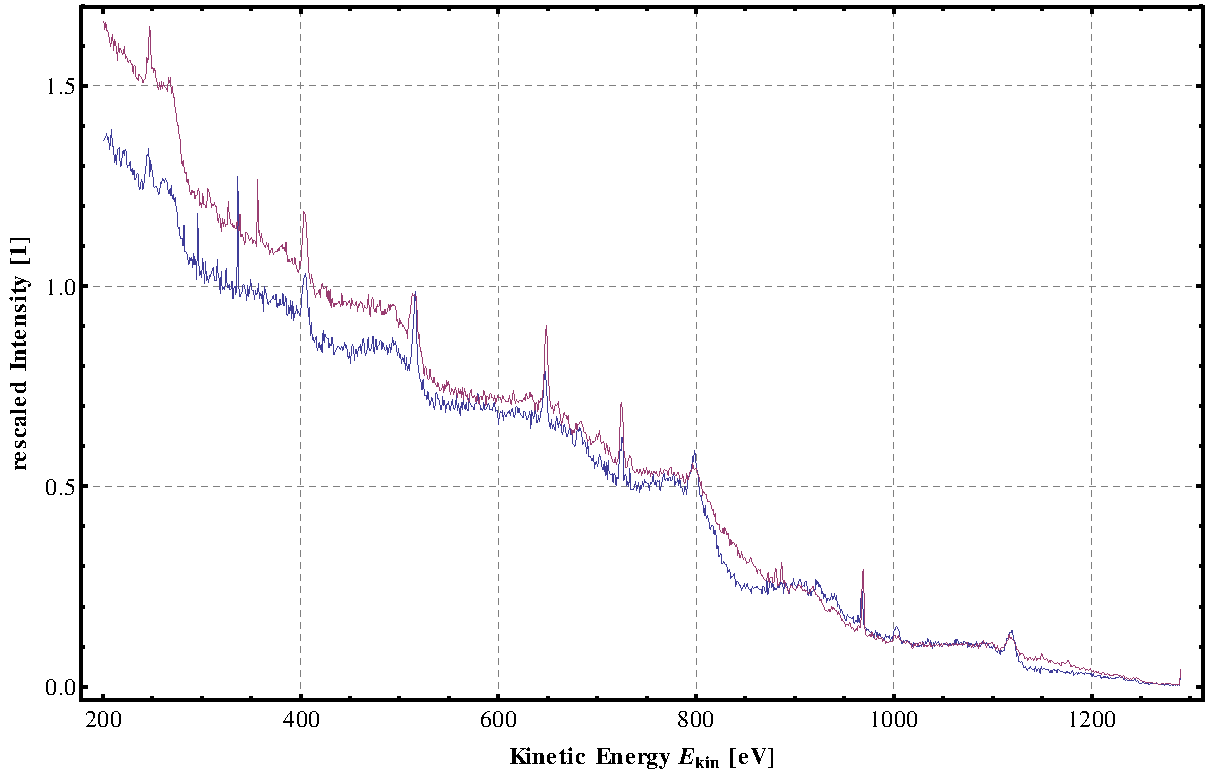
\includegraphics[scale=0.305]{img/samarium-coin_mg}
\label{fig:smc_mg}
}
\caption{Spectra for samarium and the coin, taken with aluminium anode \subref{fig:smc_al} and the magnesium anode \subref{fig:smc_mg}, rescaled to have approximately the same height. \label{fig:sm-coin}}
\end{figure}


\nocite{skript}
\nocite{handbook}
\nocite{booklet}
\nocite{nist}

\bibliographystyle{plainnat}
\bibliography{xps}

\end{document}
